\title{プロジェクトで発生するリスクのMBTI を用いた事前予測}
\author{プロジェクトマネジメントコース\\
ソフトウェア開発管理グループ\\
矢吹研究室\\
1442085\\
中村真悟}
\date{}
\begin{document}
\maketitle

%本テンプレートの余白は,卒論マニュアルで指示されたものとは違っているが,1ページあたりの文字数は40文字x40行と,卒論マニュアル通りになっている.文字間隔や行間隔を調整して,余白をマニュアル通りにすることもできるが,それでは文章が読みにくくなるため,このような対応をしている.

%\noindent
□□□□□□□□□■□□□□□□□□□■□□□□□□□□□■□□□□□□□□□■
□□□□□□□□□■□□□□□□□□□■□□□□□□□□□■□□□□□□□□□■
□□□□□□□□□■□□□□□□□□□■□□□□□□□□□■□□□□□□□□□■
□□□□□□□□□■□□□□□□□□□■□□□□□□□□□■□□□□□□□□□■
□□□□□□□□□■□□□□□□□□□■□□□□□□□□□■□□□□□□□□□■
□□□□□□□□□■□□□□□□□□□■□□□□□□□□□■□□□□□□□□□■
□□□□□□□□□■□□□□□□□□□■□□□□□□□□□■□□□□□□□□□■
□□□□□□□□□■□□□□□□□□□■□□□□□□□□□■□□□□□□□□□■
□□□□□□□□□■□□□□□□□□□■□□□□□□□□□■□□□□□□□□□■
□□□□□□□□□■□□□□□□□□□■□□□□□□□□□■□□□□□□□□□■
□□□□□□□□□■□□□□□□□□□■□□□□□□□□□■□□□□□□□□□■
□□□□□□□□□■□□□□□□□□□■□□□□□□□□□■□□□□□□□□□■
□□□□□□□□□■□□□□□□□□□■□□□□□□□□□■□□□□□□□□□■
□□□□□□□□□■□□□□□□□□□■□□□□□□□□□■□□□□□□□□□■
□□□□□□□□□■□□□□□□□□□■□□□□□□□□□■□□□□□□□□□■
□□□□□□□□□■□□□□□□□□□■□□□□□□□□□■□□□□□□□□□■
□□□□□□□□□■□□□□□□□□□■□□□□□□□□□■□□□□□□□□□■
□□□□□□□□□■□□□□□□□□□■□□□□□□□□□■□□□□□□□□□■
□□□□□□□□□■□□□□□□□□□■□□□□□□□□□■□□□□□□□□□■
□□□□□□□□□■□□□□□□□□□■□□□□□□□□□■□□□□□□□□□■
□□□□□□□□□■□□□□□□□□□■□□□□□□□□□■□□□□□□□□□■
□□□□□□□□□■□□□□□□□□□■□□□□□□□□□■□□□□□□□□□■
□□□□□□□□□■□□□□□□□□□■□□□□□□□□□■□□□□□□□□□■
□□□□□□□□□■□□□□□□□□□■□□□□□□□□□■□□□□□□□□□■
□□□□□□□□□■□□□□□□□□□■□□□□□□□□□■□□□□□□□□□■
□□□□□□□□□■□□□□□□□□□■□□□□□□□□□■□□□□□□□□□■
□□□□□□□□□■□□□□□□□□□■□□□□□□□□□■□□□□□□□□□■
□□□□□□□□□■□□□□□□□□□■□□□□□□□□□■□□□□□□□□□■
□□□□□□□□□■□□□□□□□□□■□□□□□□□□□■□□□□□□□□□■
□□□□□□□□□■□□□□□□□□□■□□□□□□□□□■□□□□□□□□□■
□□□□□□□□□■□□□□□□□□□■□□□□□□□□□■□□□□□□□□□■
□□□□□□□□□■□□□□□□□□□■□□□□□□□□□■□□□□□□□□□■
□□□□□□□□□■□□□□□□□□□■□□□□□□□□□■□□□□□□□□□■
□□□□□□□□□■□□□□□□□□□■□□□□□□□□□■□□□□□□□□□■
□□□□□□□□□■□□□□□□□□□■□□□□□□□□□■□□□□□□□□□■
□□□□□□□□□■□□□□□□□□□■□□□□□□□□□■□□□□□□□□□■
□□□□□□□□□■□□□□□□□□□■□□□□□□□□□■□□□□□□□□□■
□□□□□□□□□■□□□□□□□□□■□□□□□□□□□■□□□□□□□□□■
□□□□□□□□□■□□□□□□□□□■□□□□□□□□□■□□□□□□□□□■
■■■■■■■■■■■■■■■■■■■■■■■■■■■■■■■■■■■■■■■■
□□□□□□□□□■□□□□□□□□□■□□□□□□□□□■□□□□□□□□□■%文字数チェック用

\tableofcontents%目次

\chapter{序論}

当研究ではMBTIを用いて,メンバのタイプがプロジェクトにどのような影響を与えているかを調べることである.

\chapter{背景}

MBTI(Myers-Briggs Type Indicator)という自己理解メソッドがある.MBTIとはカール・グスタフ・ユングの心理学的類型論の指標(内向:I-外向:E,感覚:S-直感:N,思考:T-感情:F)に判断的態度:J-知覚的態度:Pの指標を加えて,4指標16タイプとして性格を分類する.主に相談場面や教育現場,企業の組織編制,人事政策などに利用されている\cite{110001230195}.

このMBTIを使い,プロジェクトの開始時点からメンバの性格を理解し,メンバの相互作用が原因となって起こる事象を予測したい.本研究ではMBTIを用いて,グループワークでの事象とメンバの性格との相関関係について研究する.

\chapter{MBTIについて}

MBTIとは正式名Myers-Briggs Type Indicatorと言われる.人の心の癖をくみ取ることを目的に作られた.MBTIは,カール・グスタフ・ユングの心理学的類型論の指標(内向:I-外向:E,感覚:S-直感:N,思考:T-感情:F)に判断的態度:J-知覚的態度:Pの指標を加えて,4指標16タイプとして性格を分類する.

\newpage
\section{外向:Eと内向:I}
どんなものに興味を持ち,やる気を出すかが傾向として出る.

外向:Eとは以下の傾向がみられる.
\begin{itemize}
\item 自分の周囲で起きていることに注意を払う
\item 話すことによるコミュニケーションをより好む
\item 実際に行動したり,人との関わりを通じて,学ぶ
\item 興味を広げる
\item 人と話をしながら考え,まとめていくことが多い
\item 人との交流を好み,自分を表現することが多い
\item すすんで周囲の人や出来事に関わっていく
\end{itemize}

内向:Iとは以下の傾向がみられる.
\begin{itemize}
\item 自分の内面に起きている事に注意を払う
\item 書くことによるコミュニケーションをより好む
\item 内省したり,肉体的体験を通じて,学ぶ.
\item 興味を掘り下げる
\item 考えがまとまってから話すことが多い.
\item 一人でいることを好み,自分を表現することが少ない
\item 今していることに集中して取り組んでいく
\end{itemize}


\newpage
\section{感覚:Sと直感:N}

どのように情報を取り入れるのかが傾向として出る.

感覚:Sとは以下の傾向がみられる.
\begin{itemize}
\item 実際に今起きていることに着目する
\item 実際に役立つことや実践的なことに価値を置く
\item ひとつひとつ具体的なことに重きを置く
\item ものごとを観察したり,記憶する.
\item 先のことより,今に目が向きやすい
\item ひとつずつ,順を追いながら情報を集める
\item 経験の積み重ねを信頼する
\end{itemize}

直感:Nとは以下の傾向がみられる.
\begin{itemize}
\item ものごとの全体像や可能性に着目する.
\item イメージや洞察に価値を置く
\item 抽象的なことや理論を大切にする
\item 事実の背景にあるパターンや意味をとらえる
\item 今より先のことに眼が向きやすい
\item ふっと思いついたり,思いたったことなどから情報を集める
\item ひらめいたことを信頼する
\end{itemize}
\newpage
\section{思考:Tと感情:F}

どのように結論に導くことを好むのかが傾向として出る.

思考:Tとは以下の傾向がみられる.
\begin{itemize}
\item 分析的観点を重視して考える
\item 論理的に課題を解決に導く
\item 原因と結果から考える
\item 毅然とした印象を与える
\item 気持ちに左右されず,客観的な真実を追究する
\item 合理性を大切にする
\item 公平である
\end{itemize}

感情:Fとは以下の傾向がみられる.
\begin{itemize}
\item 相手や自分の大切にしていることを重視して考える
\item 人々への影響を考慮する
\item 自分の価値基準から考える
\item 親しみやすい印象を与える
\item 調和や個人の尊重を求める
\item 気持ちを大切にする
\item 受け入れる
\end{itemize}

\newpage
\section{判断的態度:Jと知覚的態度:P}

どのように外の世界と接することを好むかが傾向として出る.

判断的態度:Jとは以下の傾向がみられる.
\begin{itemize}
\item スケジュールにそって行動する
\item 整理された状態を好む
\item 規律正しい
\item どちらかというと几帳面な
\item まずは計画を立てる
\item 結論を出すことや決着をつけることを好む
\item 最後に慌ててやることを避ける
\end{itemize}

知覚的態度:Pとは以下の傾向がみられる.
\begin{itemize}
\item 状況に応じて行動する
\item 制約にとらわれない
\item 格式ばらない
\item どちらかというと柔軟な
\item まずは状況をみる
\item 結論や結果に変更の余地を残しておくことを好む
\item 最後に一気にやる
\end{itemize}
\newpage

\section{MBTIのタイプについて}
以上の4指標2傾向で表される.2の4乗の組み合わせで16タイプになる.
\subsection{ISTJ}
実直で,静かで,集中して几帳面にものごとをやり遂げる.
実践的で,秩序や事実を重視し,論理的,現実的で,頼みにできる.
すべてを体系立てて整理しようとする.
責任感があり,やるべきことをいったん決めたら,抵抗や障害にあっても着実にやり通す.
\subsection{ISTP}
冷静な観察者.
口数が少なく,人に自ら働きかけることはあまり多くない.
対象から距離を置いたところで好奇心があり,周囲が予期しないような独自のユーモアセンスをもって,ものごとを観察し,分析する.原因と結果や,メカニズム,論理的な原則に基づく事実の体系づけに興味を示す.身近な問題の核心をとらえ,解決策を見つける.
\subsection{ISFJ}
静かな方で,友好的で,責任感があり,実直である.義務を果たそうと誠心誠意尽くす.
課題遂行やグループ活動に着実さをもたらす.
几帳面で,労をいとわず,ものごとに正確である.技術的なことにはあまり興味を示さない.
忍耐強く,ものごとの詳細に取り組む.
人に対して忠実で,思いやりがあり,感覚が鋭く,相手の気持ちを大切にする.
\subsection{ISFP}

遠慮深く,もの静かで,友好的である.また,人の気持ちに敏感で,人当たりもソフトで,謙遜な態度を示す.
不和を避け,自分の意見や価値観を他者に押し付けないようにする.周囲を進んで引っ張っていくより,支持する側にまわることが多い.
今を実際に楽しんだり,味わったりすることを大切にし,あわてたり無理をすることを好まないため,気張らずにものごとを行うことが多い.
\newpage

\subsection{INTJ}
独自の考え方をもち,自分のアイデアや目的の追求に高い関心をもっている.長期的な視野をもち,出来事の意味やパターンを素早く見出す.自分が興味ある分野においては,体系立てて課題を整理し,最後までやり遂げようとする.
懐疑的,批評的,自立的で,堅い決意をもつ.
能力や成果に高い水準を求める.
\subsection{INTP}
口数が少なく,人と進んで関わるより,理論的,科学的な探求に楽しみを見つける.
いろいろなアイデアに興味を持ち,社交的な集まりや,とりとめのないおしゃべりには,あまり関心を示さないことが多い.自分の興味がはっきりしていることが多く,自分の中にある興味を生かしたり,役立たせることが可能な職業を求める.
\subsection{INFJ}
忍耐強く,独自性があり,自分に求められていることや,望まれていることに応えるために意欲をもって,最善を尽くそうとする.
控えめながら,押しが強く,実直で,他者を気遣う.強い信念にもとづいて,世の中に貢献するための明確な視野をもつことにより,信望を得ることがある.
\subsection{INFP}
静かな観察者で,理想を求め,人に忠実である.外で起きていることと,自分の内面の価値観と一致していることを重視する.
好奇心があり,ものごとの可能性を素早く見出し,アイデアを実行に移す促進者の役割をとることが多い.
順応性,柔軟性があり,自分の価値観がおびやかされない限り,受容的な態度を示す.人を理解したり,人間の可能性を実現する方法を求める.
所有物や物理的環境にはあまり関心を払わない.
\newpage

\subsection{ESTJ}
経験的に思考し行動する.
現実や実際的なことを重視し,経営や機械工学などに興味関心をもつ.
抽象的な理論を学ぶよりも,論理的に体系立てたことを実際にすみやかに遂行しうるように習熟しようとする.
決断性があり,決定を素早く実行に移し,一つ一つ確実に積み重ねながら,実際に運営したり,事を動かすことに力を発揮する.
\subsection{ESTP}
自分の置かれた状況の問題を,直接解決していくことに力を発揮する.実際い行動することを好み,来るものは拒まずの精神で楽しむ.
メカニックスを扱ったり,友人や知人と共にスポーツや活動をすることを好む.順応性があり,許容範囲が広く,具体的な効果や結果を得ることに関心を払う.
冗長な説明を嫌い,具体的なものやことがらを直接扱ったり,操作・分解,組み立てることに力を発揮する.
\subsection{ESFJ}
親しみやすく,おしゃべりを好み,実直で,生まれながらの協力者,または熱心な活動家である.
調和を求め,それを創りあげることを好んでする.快活で,人のためになることをしようとし,励まされたり,ほめられることで力を発揮する.
直接目にみえた形で,人の生活に影響をおよぼすものに高い関心を持つ.
\subsection{ESFP}
人やできごとなど外界と関わることを好み,受容的,友好的で,あらゆることに楽しみを見つけ,他者がより楽しめるように,工夫することに喜びを見出す.
体を動かして行動することや,周囲に働きかけることを好み,今起こっていることに目を向け,意欲をもって参加していく.
理論をマスターするよりも,実際に体験しながら覚える方が楽に感じることが多い.常識や実践的な対人能力が必要とされる場面で,力を発揮する.
\newpage

\subsection{ENTJ}

思弁的に思考し行動する.率直な態度と,決断性をもつリーダー的存在であることが多い.組織の問題を解決するために必要な,統合的なシステムをつくり,それを実際に導入しようとする.

弁論のような,論理的で知的な話をすることを好む.常にさまざまな情報に通じており,知識の蓄えを増やしていくことに楽しみを見つける.
\subsection{ENTP}

反応が素早く,独創的で,得意なことが多い.周囲に刺激を与え,機敏で,率直である.

賛成,反対のどちら側からも,楽しんで議論に加わることが多い.未知のことや,挑戦的な問題解決に対して臨機応変に対処するが,定型作業を軽視することがある.次々に新しいことや考えに掻き立てられ,自分のしたいことに,論理的なaikani理由を見出す.
\subsection{ENFJ}

周囲の状況に敏感に反応し,責任ある行動を取る.

他者の考えや期待されていることを心から気遣いながら,ものごとに対処しようとする.提案をしたり,グループの進行を,そつなく巧みに行うことが多い.
社交的で,思いやりがあり,周囲の賞賛や批判に敏感である.
人の手助けをすることを好み,人の成長を可能にしようとする.
\subsection{ENFP}

人あたりがよく,快活で,情熱的で,意気盛んにものごとに関わり,独創的で,想像力に富んでいる.興味が起きれば,どのようなこともすることができる.

難しいことへの解決法を素早く思いつき,困っている人を助けられる態勢にあろうとする.事前に準備しておくよりも,即興で対応することが多い.自分のしたいことに,どうしてもそれをせざるを得なくなるような理由を見つける.
\newpage

\section{現在の活用法}
主に相談場面や教育現場,企業の組織編制,人事政策などに利用されている\cite{110001230195}.

アメリカでは,日本の血液型を聞く文化と同じようにタイプを訪ねる文化がある.キャリアコンサルティングにも導入されており,自分のタイプと適性があるといわれている職業のリストを用いてコンサルティングする.


\begin{figure}[thbp]
   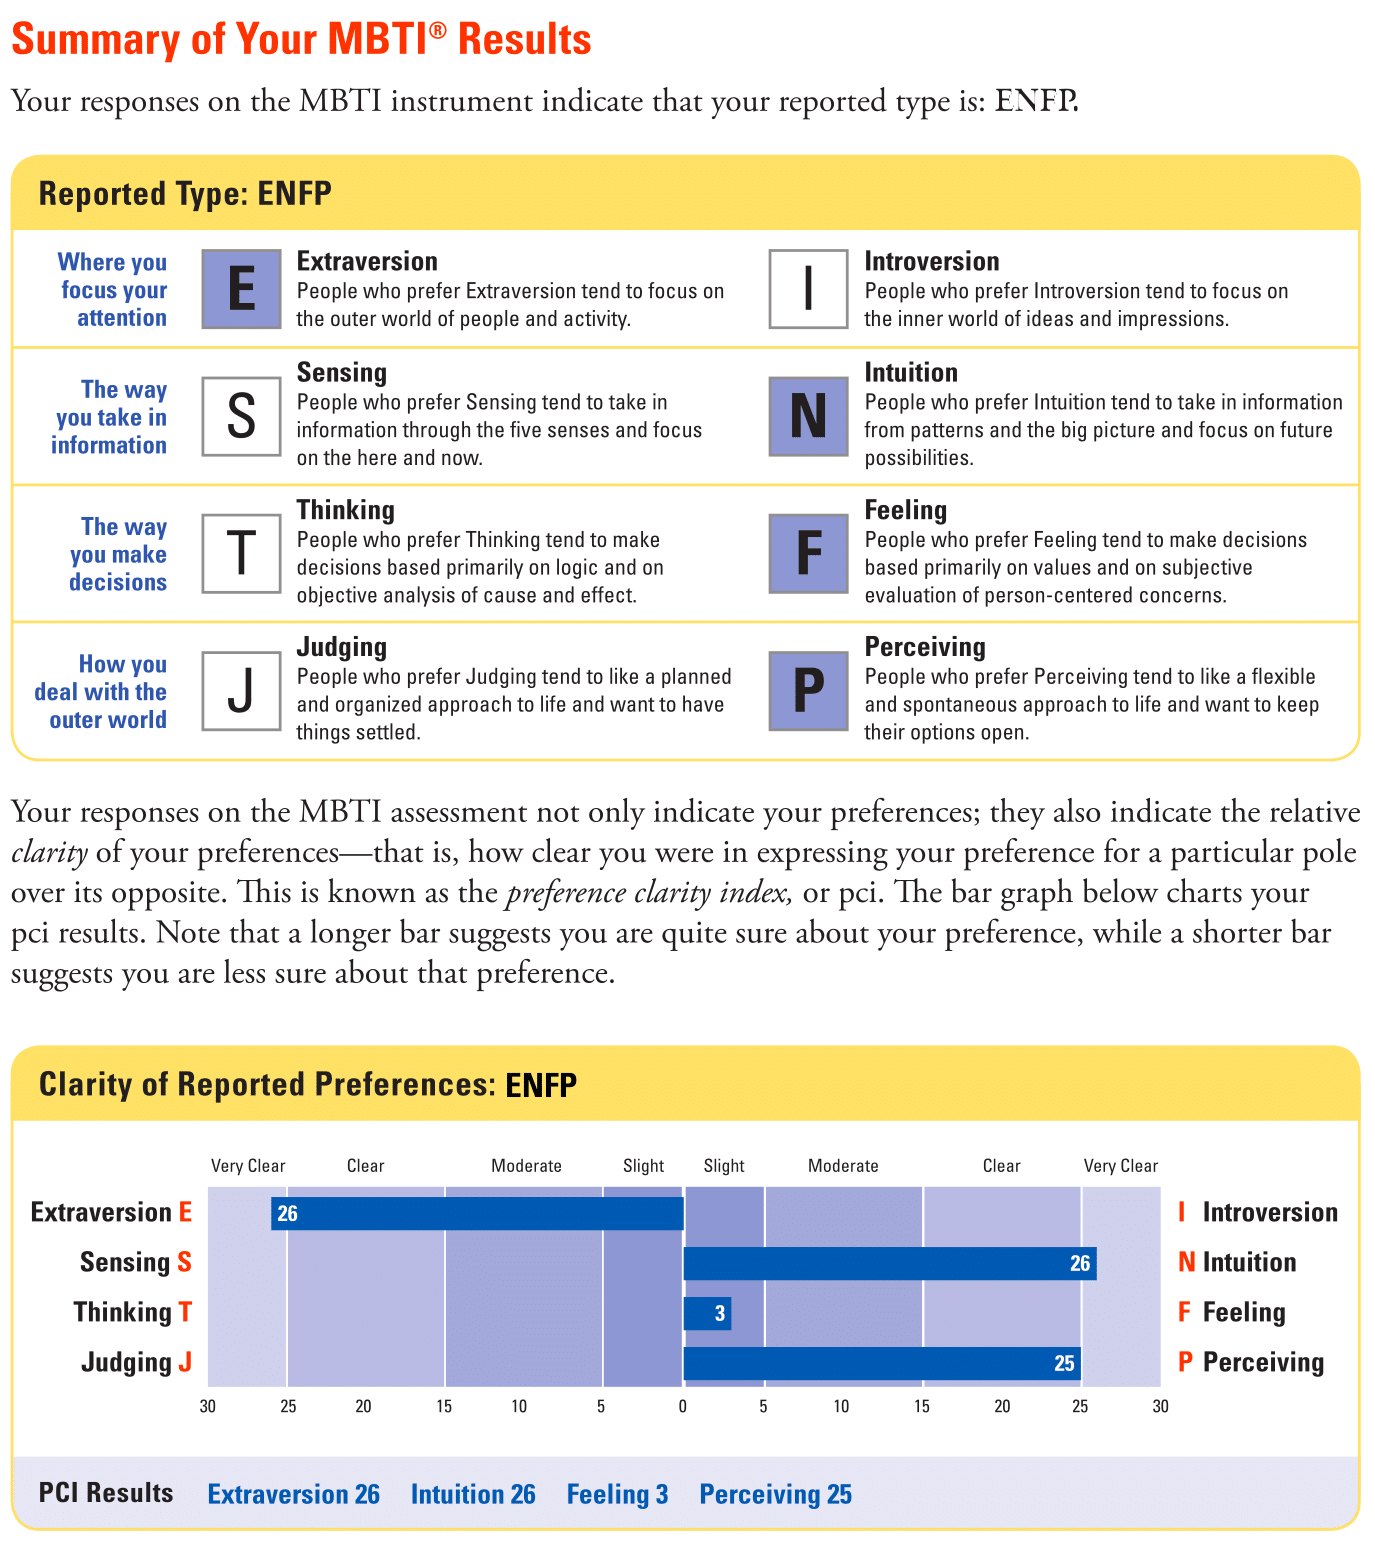
\includegraphics[width=13cm]{mbti1.png}
   \caption{MBTIの診断結果}
   \label{M}
\end{figure}

\nocite{kaigai}

\chapter{目的}
本研究の目的は,メンバのMBTIのタイプの相互作用がプロジェクトのリスクにどう影響を及ぼしているのかを調べ,メンバ間で発生しやすいリスクを予測することである.


\chapter{手法}
以下の手法で研究する.
\begin{enumerate}
\item グループワークで課題に取り組んでもらう.
\item グループワーク後に,性格検査と発生したリスクについてのアンケートを行う.
\item 集めた回答結果をトレーニング用とテスト用にデータを分ける.
\item トレーニング用データをアソシエーション分析し,確信度が一定の値(閾値)を超えたルールを採用する.
\item テストデータを使い,ルールの精度と再現率(後述)を求める.
\item 精度と再現率の調和平均(F値)を求め,値が最も高くなるルール抽出の閾値を求める.
\end{enumerate}


\newpage
\section{PM実験について}
千葉工業大学で開講される講義である.

15週の講義を半分に分けて行い,6週で簡易化されたプロジェクトをグループで行ってもらう.二つのコースがあり,新規ビジネスを企画し提案するビジネス創成コースとテーマを決めホームページを作るソフトウェア開発コースがある.
\section{PM演習について}
千葉工業大学で開講される講義である.

15週の講義を簡易化されたプロジェクトをグループワークとして行ってもらう.PM実験同様二つのコースがあり,新規ビジネスを企画し利益などコストの試算を行い,実現性を深めて提案するビジネス創成コースとテーマを決め,webアプリケーションを作るソフトウェア開発コースがある.
\newpage
\section{プログラミング言語とプログラミングについて}
千葉工業大学で開講される講義である.
\subsection{授業の目的}

ソフトウェア開発は,要件定義や設計,プログラミング,テストなどの工程からなる.

本講義では,この中のプログラミングに焦点を当て,その活動の全体像を理解することを目指す.プログラマを目指す学生だけでなく,将来ソフトウェア開発に携わる可能性のあるすべての学生を対象に,プログラムを書けるようになるというよりは,プログラムを書くということがどういうことなのかがわかるようになるための講義を行う.

\section{データマイニング入門ついて}
千葉工業大学で開講される講義である.
\subsection{授業の目的}

データマイニングとは,大量のデータから有用な情報を取り出す手法の総称である.データマイニングの知識や技術は,デジタル化されたデータが大量に蓄積され「ビッグ・データ」などと呼ばれる今日において,とても重要である.

本講義では,データマイニングのさまざまな手法について学び,表計算ソフトウェアと統計処理専用ソフトウェアで実際にそれを実現する技術を獲得することを目指す.

\subsection{データマイニングとは}

データマイニングとは,1990 年代中頃から用いられるようになった言語であり,統計学,人工知能などのデータ解析の技法を用いて,多くのデータから知識を取り出す技術のことである.データマイニングの適用分野や目的,対象となるデータの種類は多種多様である.

ビジネスの分野では企業が業務に関連して記録したデータ(過去の行動履歴,取引記録など)を元に,意思決定や計画立案,販売促進などに有効な知見を得るために行われることが多い.

\subsection{データマイニングの事例}
1992年12月23日,米紙『ウォールストリートジャーナル』に掲載された,「Supercomputer Manage Holiday Stock」という記事がすべての始まりと言われている.

「米国の大手スーパーマーケット・チェーンで販売データを分析した結果,顧客はビールとおむつを一緒に買う傾向があることがわかった.調査の結果,子供のいる家庭では母親はかさばる紙おむつを買うよう父親に頼み,店に来た父親はついでに缶ビールを購入していた.そこでこの2つを並べて陳列したところ,売り上げが上昇した.」

このようにデータマイニングの結果から推測することで顧客の潜在的なニーズを引き出すことができる.
\newpage
\subsection{グループワークの内容}

PM実験・演習は講義全体がグループワークとなっている.
\subsection{データマイニング入門}

期間:4週間

 第1,2週

  グループ内でテーマとマイニング方法を二つ決める

  テーマに応じた質問をグループの人数分作成する

 第3,4週
 
  アンケートのデータをマイニングする

  グループ内のデータで結果が出ない場合,他のグループのアンケート結果を用いる

  結果と考察
\nocite{ylab2015}
\newpage
以降はアンケートの一部である.
\begin{figure}[thbp]
   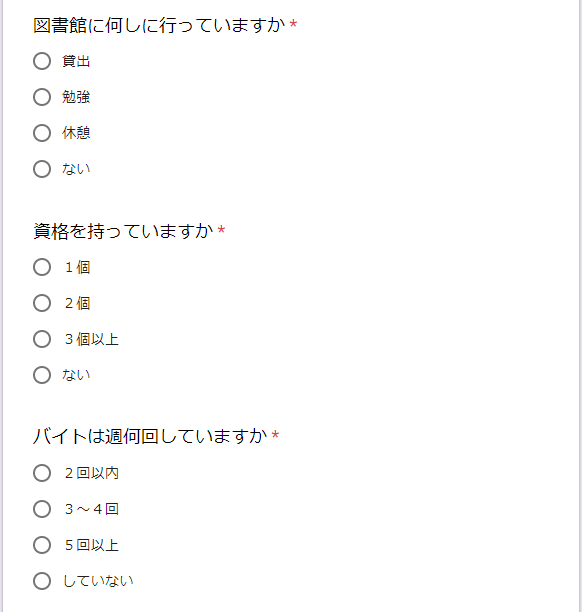
\includegraphics[width=13cm]{dma1.png}
   \caption{学生が考えたアンケート}
   \label{M}
\end{figure}

\newpage
\begin{figure}[thbp]
   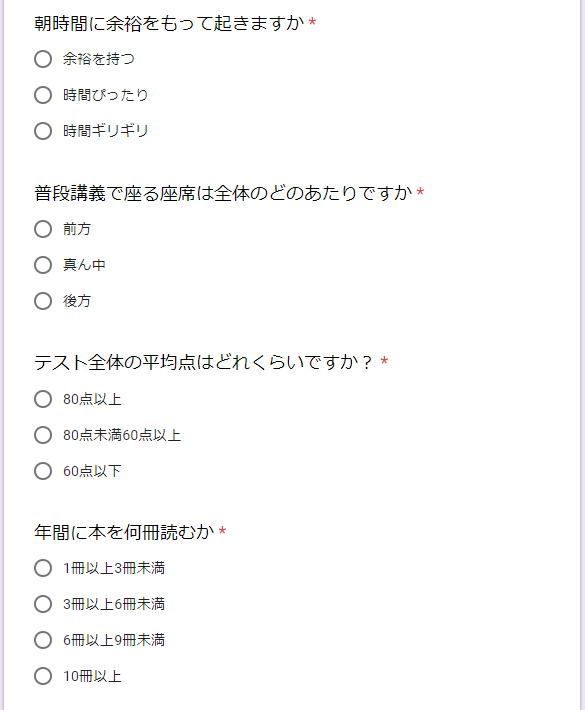
\includegraphics[width=13cm]{dma2.png}
   \caption{学生が考えたアンケート}
   \label{M}
\end{figure}

\newpage
\begin{figure}[thbp]
   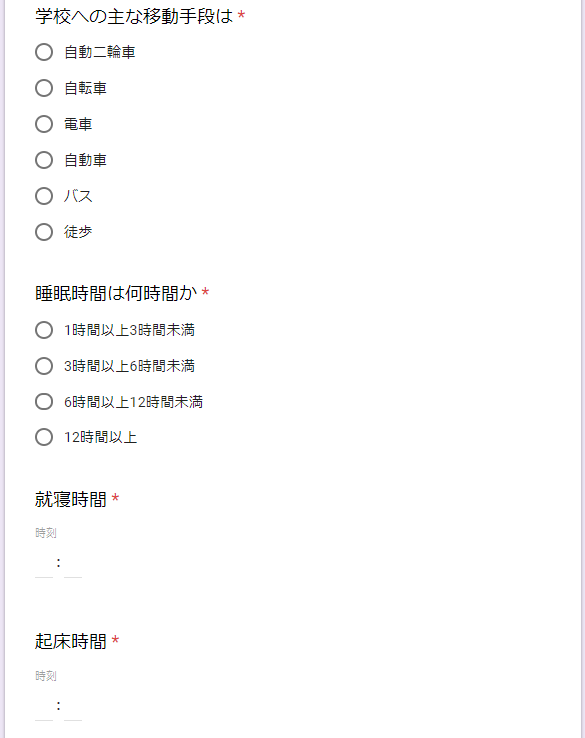
\includegraphics[width=13cm]{dma3.png}
   \caption{学生が考えたアンケート}
   \label{M}
\end{figure}
\newpage







\subsection{プログラミング言語とプログラミング・情報リテラシ}

期間:5週間
 第1週

  グループ分け

 第2~4週

  調査・報告用動画作成

 第5週

  課題提出

\newpage

\section{Googleフォームについて}
Googleフォームとは,Googleドライブ上のサービスの一つである.

\begin{figure}[!htbp]
\centering 
\includegraphics[width=13cm]{Gformkai.png}
\caption{回答者が見るページ}
\end{figure}
\newpage
アンケートフォームを簡単に作成することができ,回答結果は円グラフにて表示される.
\begin{figure}[!htbp]
\centering 
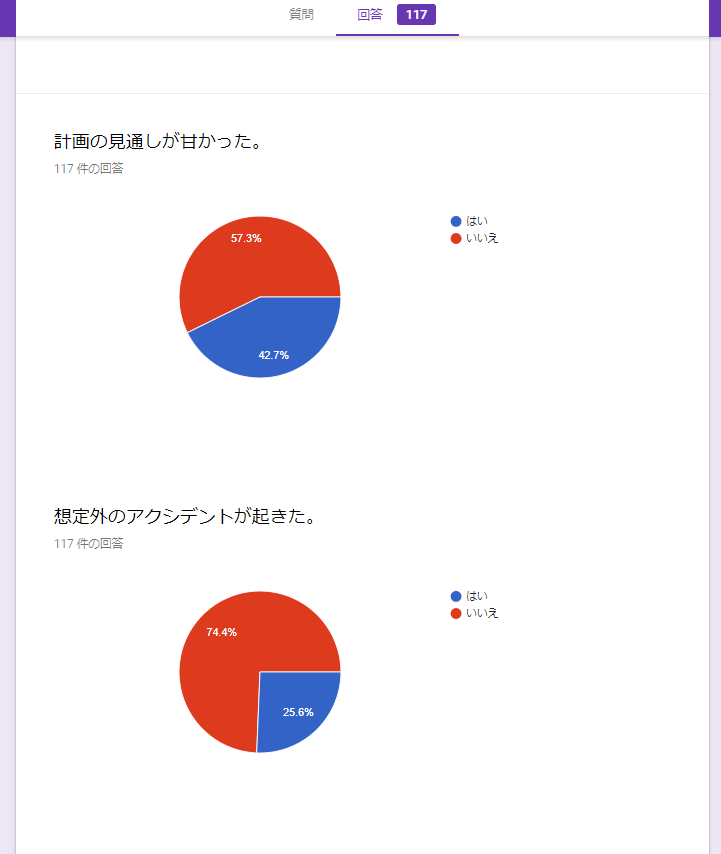
\includegraphics[width=13cm]{Gforman.png}
\caption{回答結果の円グラフ}
\end{figure}
\newpage
また,回答結果はCSVファイルでダウンロードし,オフラインでもデータを利用することができる.
\begin{figure}[!htbp]
\centering 
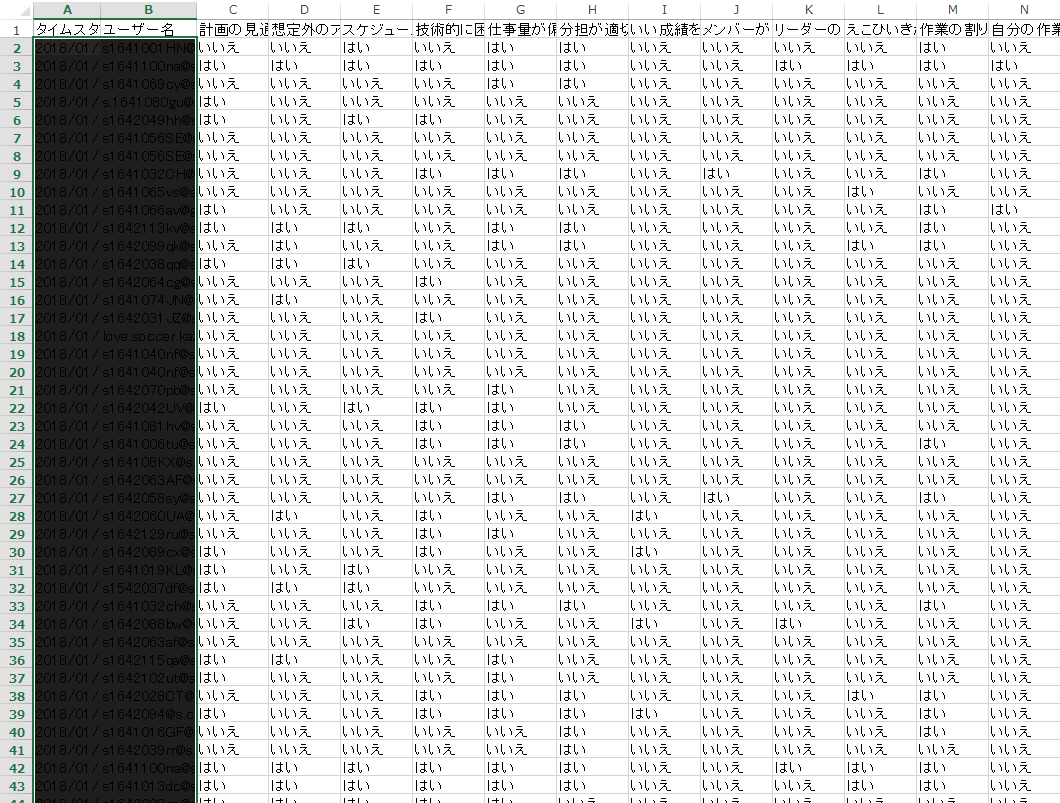
\includegraphics[width=13cm]{GFcs.png}
\caption{回答結果のCSVファイル}
\end{figure}
\newpage

\section{性格検査について}
\subsection{性格検査}
今回行った性格検査はGoogleフォームを用いた.

質問内容は「性格学入門―運命のカギをにぎる16のタイプ別性格判断」の簡易MBTI診断をそのまま使用している\cite{MBTI}.質問は選択肢で「はい」と「いいえ」の二択で回答する.

内容は次のとおりである.
\begin{itemize}
\item 自分の意見を聞かれたときに,しっかり頭で考えてから話すより,口に出しながら考えていくほうだ.
\item 自分に興味のないテレビやCDがかかっている場所でも,平気で本を読んだり人と話ができる.
\item 自分の性格や,やっている仕事などについて人からどう思われているか,つねに他人の目が気になる.
\item 相手が初対面の人間でも,知り合いに対するようのと同じようにリラックスして話し掛けることができる.
\item 物事を決めるときには,自分一人で決めるのではなく,必ず誰かに相談して決める.
\item 人の話を黙って聞いているのが苦手で,会議で誰かが話していてもつい口をはさんでしまうことがある.
\item 物を捜していたり自分にはわからない事柄がある時には,自分で調べる前にまず人に聞いてしまう.
\item 人にお世辞を言うのも,人からお世辞を言われるのも,別にそれほどいやだとは思わない.
\item 仕事に没頭しているときでも,途中で電話や呼び出しがかかれば,すぐに手を止めて対応できる.
\item 時間を尋ねたときに,「4時ちょっと前」のようなあいまいな答え方をされるといらいらする.
\item 機械や道具が少しぐらい壊れていても,実際の使用にさしさわりなければ別に気にならない.
\item 着想や理論がいくら優れていても,数字や事実関係の裏づけのない企画は評価できない.
\item 雑誌を読むときは,大抵最初のページから順番に読んでしまう.
\item 人のいうことを額面どおりに受取りやすく,言葉の裏に隠された意味を考えるのは苦手だ.
\item 多少遅れてもかまわないようなパーティーでも,律儀に時間どおりに行かないと気がすまない.
\item 月末に残高が少なくなると,次の給料の使い道よりも,それまでのやりくりのほうを考えてしまう.
\item 自分の担当の仕事をしているだけで楽しく,職場全体の中での役割や立場まで気が回らない.
\item たとえオフィスの掃除のようなことでも,目に見える形で結果が出る仕事にはやりがいを感じてしまう.
\item 多少は自分が無理をしてでも,その場の雰囲気や周りの人の思惑に合わせてしまうほうだ.
\item 決定的な対立が起こりそうな時,一時しのぎとわかっていても衝突を避けることを考えてしまう.
\item 何かを決める場合,理屈の上で正しいかどうかよりも,誰もが納得するかどうかのほうが重要だと思う.
\item 会議などで自分に不利な意見を聞くと,自分に対する当てこすりのように感じてしまう.
\item この世には論理的なもの,科学的なものでは割り切れない物事があると信じている.
\item 自分の意見を言いたいのに,周りから気にかけられないと思うと口に出していえない.
\item 数字や番号を覚えるよりは,人の名前や顔を覚えるほうがずっと得意だ.
\item 「愛」というものは言葉で定義できないものであり,それを定義しようとする人は不愉快だ.
\item 利用されているだけではないかと思っていても,頼まれごとをされるとつい引き受けてしまう.
\item 何事にもスケジュールをしっかり立てないと気が済まず,その予定通りにいかないと不安だ.
\item 自分の意見を言っているだけなのに,よく怒っているのではないかと誤解されることがある.
\item 机の上や本棚,冷蔵庫や洋服ダンス,壁に掛けた絵など,なんでもきちんとしていないと気がすまない.
\item 何事にせよ一度始めたことは,とにかく最後までやり遂げて片付けてしまう.
\item 家から会社に行くまでのルートは毎日まったく同じコースを通って行くことにしている.
\item 人がみなやるべきことをきちんとやれば,この世はもっとよくなるに違いないと思う.
\item 締め切り間際に慌てるのはいやなので,仕事はきちんとペース配分して行うことにしている.
\item 不意打ちや予定外の行動が苦手で,状況の変化に臨機応変に対処することができない.
\item 仕事は仕事なのだから,そこに遊びの要素を求めるのはどこかおかしいと思う.
\end{itemize} 


 \newpage


\subsection{タイプ分類について}
ブラウザ上で回答結果をクリックすることによって判定可能なサイトを用いて,分類した\cite{mbtib}.
結果は表\ref{MBTI結果}のようになった.
\begin{table}
  \caption{性格検査の結果}
  \label{MBTI結果}
  \centering
  \begin{tabular}{l|r}
タイプ & 人数 \\
  \hline
ISTP & 10 \\
INTP & 13 \\
ISTJ & 5 \\
INTJ & 0 \\
ISFP & 13 \\
INFP & 7 \\
ISFJ & 11 \\
INFJ & 3 \\
ESTP & 9 \\
ENTP & 9 \\
ESTJ	 & 3 \\
ENTJ	 & 6 \\
ESFP	 & 13 \\
ENFP	 & 13 \\
ESFJ	 & 23 \\
ENFJ	 & 3 \\
 \hline
  \end{tabular}
\end{table}
 \newpage

\section{アンケートについて}

\begin{figure}[htb]
\centering
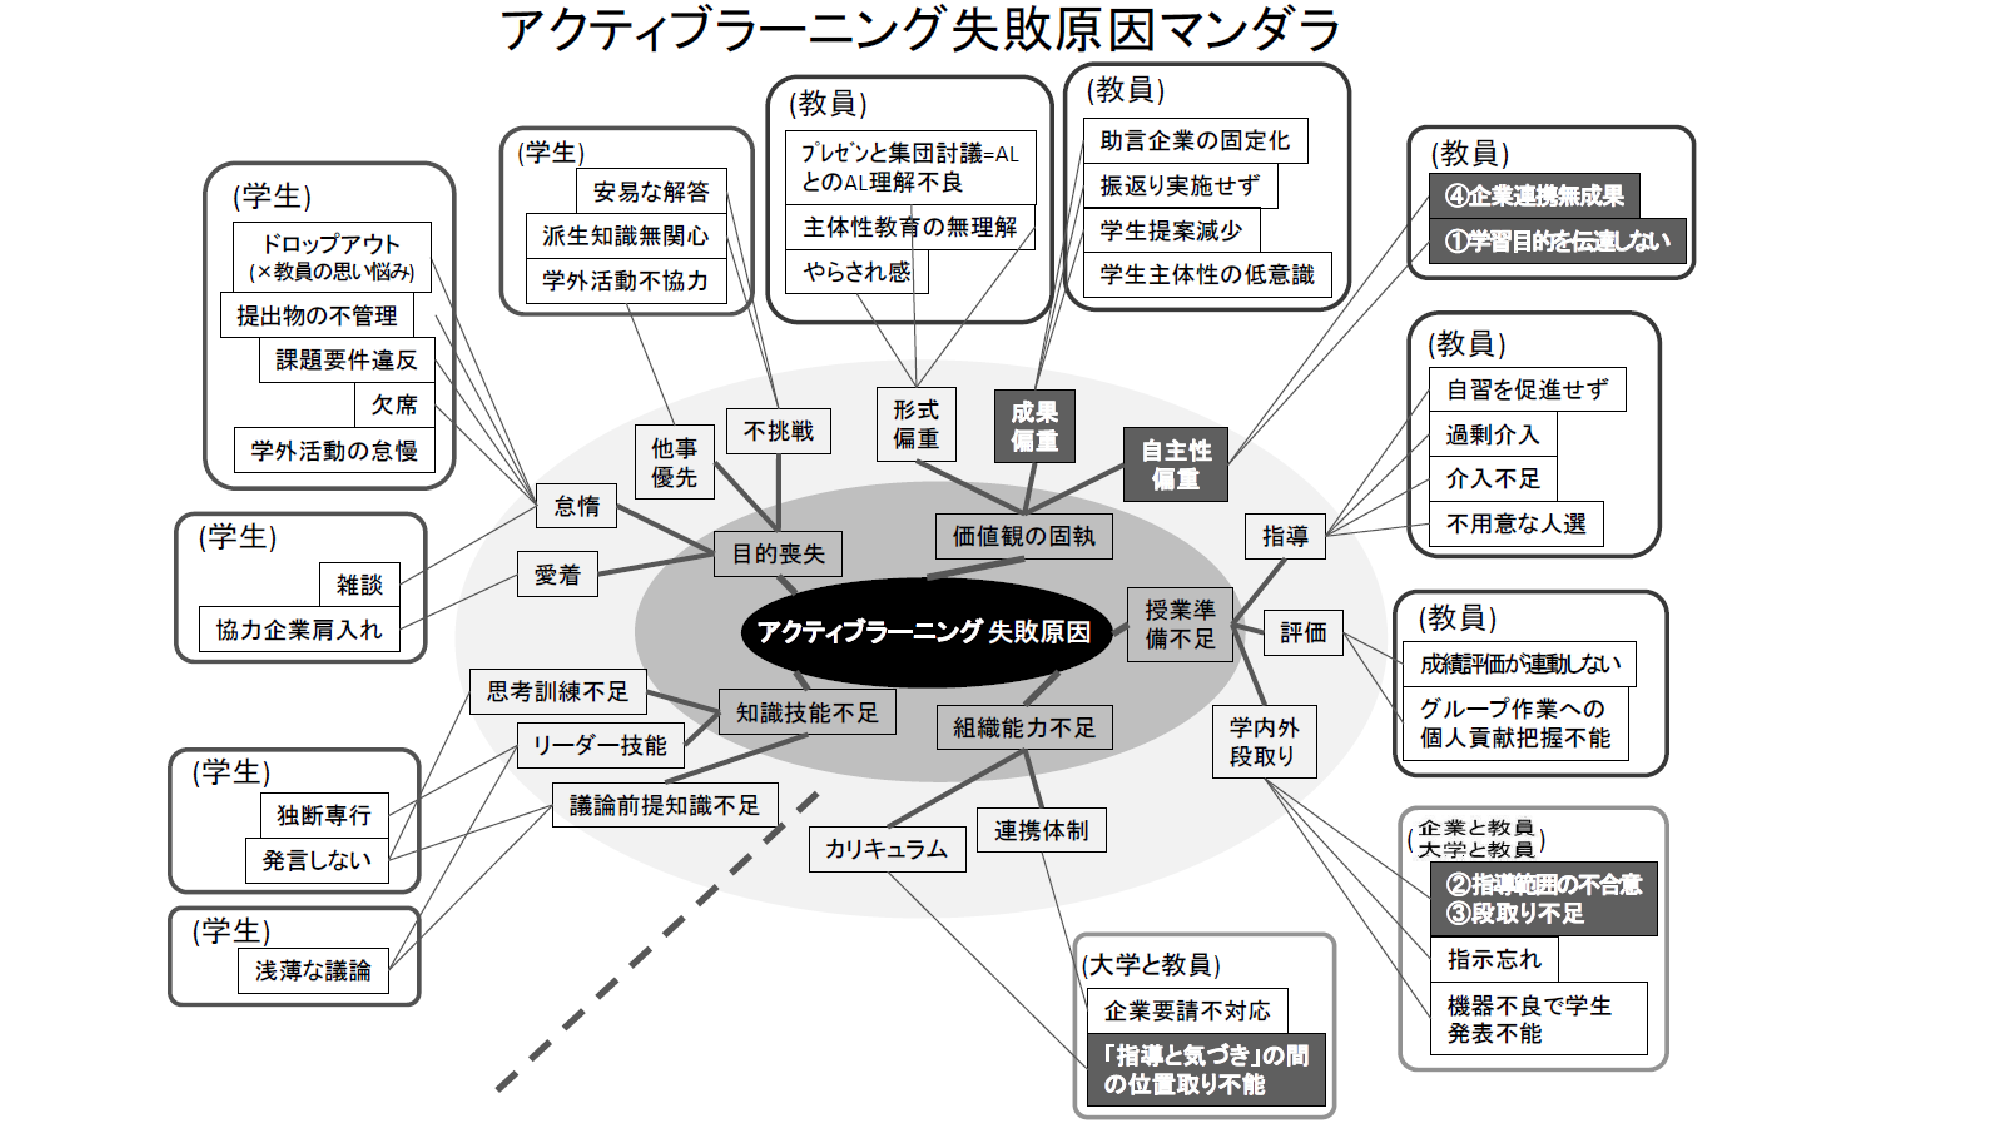
\includegraphics[width=10cm]{sippaimandara.pdf}
\caption{アクティブラーニングにおける失敗原因マンダラ}\label{失敗曼荼羅}
\end{figure}

リスクについてのアンケートは上記の失敗原因マンダラ\cite{110009915588}を参考に作成した.

アンケートの内容は次のページになる.質問はすべてはいといいえで答えるようになっている.
 \newpage
\begin{itemize}
\item 計画の見通しが甘かった.
\item 想定外のアクシデントが起きた.
\item スケジュールに遅れが出た.
\item 技術的に困難なことは他人に任せた.
\item 仕事量が偏っていた.
\item 分担が適切ではなかった.
\item いい成績を取るという意欲はなかった.
\item メンバーが何をしたのか把握していない.
\item リーダーの指示はすべて把握していない.
\item えこひいきがあった.
\item 作業の割り振りは妥当ではなかった.
\item 自分の作業を決められた通りの期日に遅れた.
\item 進んで作業に取り組めなかった.
\item 単位を取れればいいやという気持ちはあった.
\item メンバーと前より仲が悪くなった.
\item 毎週の連絡を忘れた.
\item 成果物や作業指示の確認を怠った.
\item 進捗を把握していない.
\item 間違って同じ作業をしてしまった.
\item 作業量が自分だけ多かった.
\item リーダーの指示がわかりにくかった.
\item 意見を聞いてもらえず話し合いにならないことがあった.
\item 話し合いで無言が続いた.
\item 話し合いの場で進んで発言できなかった.
\item 情報共有は問題があった.
\item チーム内で諍いが起きた.
\item 講義を休んだ.
\item リーダーの指示は的確ではなかった.
\item やらされているようであった.
\item 提出物に関係するものに不備があった.
\item 途中退席した.
\item 無断欠席した.
\item 雑談が多かった.
\item 講義に関係ないことをしていた.
\end{itemize} 


 
 
 
 
 

.



\section{Rによるデータ解析}

\subsection{R言語とは}

R言語はオープンソース・フリーソフトウェアの統計解析向けプログラミング言語(あるいはその実行環境)である.\cite{R}オープンソースであるにも関わらず,統計解析用ソフトとして十分な機能,性能を有しており,多くの研究機関や教育機関に採用されている.
\subsection{Rの導入方法}

Rのインストーラーをwebページからダウンロードする方法と,Chocolateyを利用してインストールする方法の2通りの方法を解説する.なお,解説するのはWindows版のRのみとする.

\subsubsection{インストーラーをダウンロードしてインストールする手順}

CRAN(The Comprehensive R Archive Network)が提供するR for Windowsのインストーラーダウンロードページに行く.(https://cran.ism.ac.jp/bin/windows/)今回はbaseをインストールするので,install R for the first timeを選択.

\begin{figure}[htbp]
\centering 
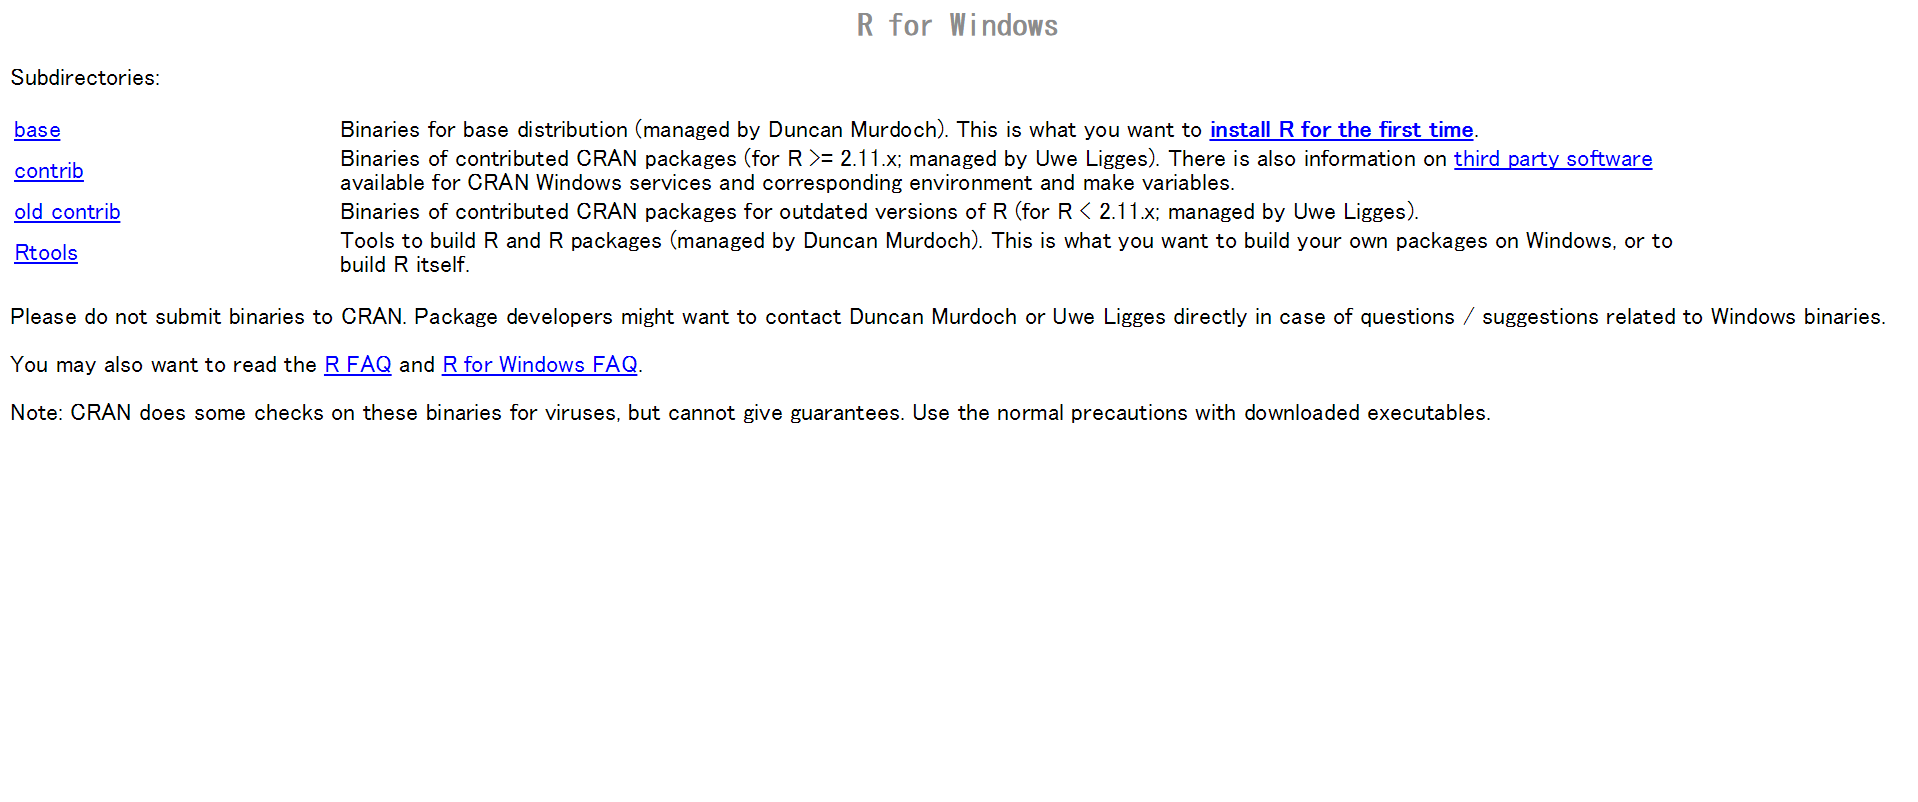
\includegraphics[width=13cm]{rinst1.png}
\caption{install R for the first timeをクリック}
\end{figure}

\newpage
ページが遷移したら,一番上のDownload R 3.3.1 for Windows(3.1.1の部分はバージョンによって異なる)をクリック.

\begin{figure}[htbp]
\centering 
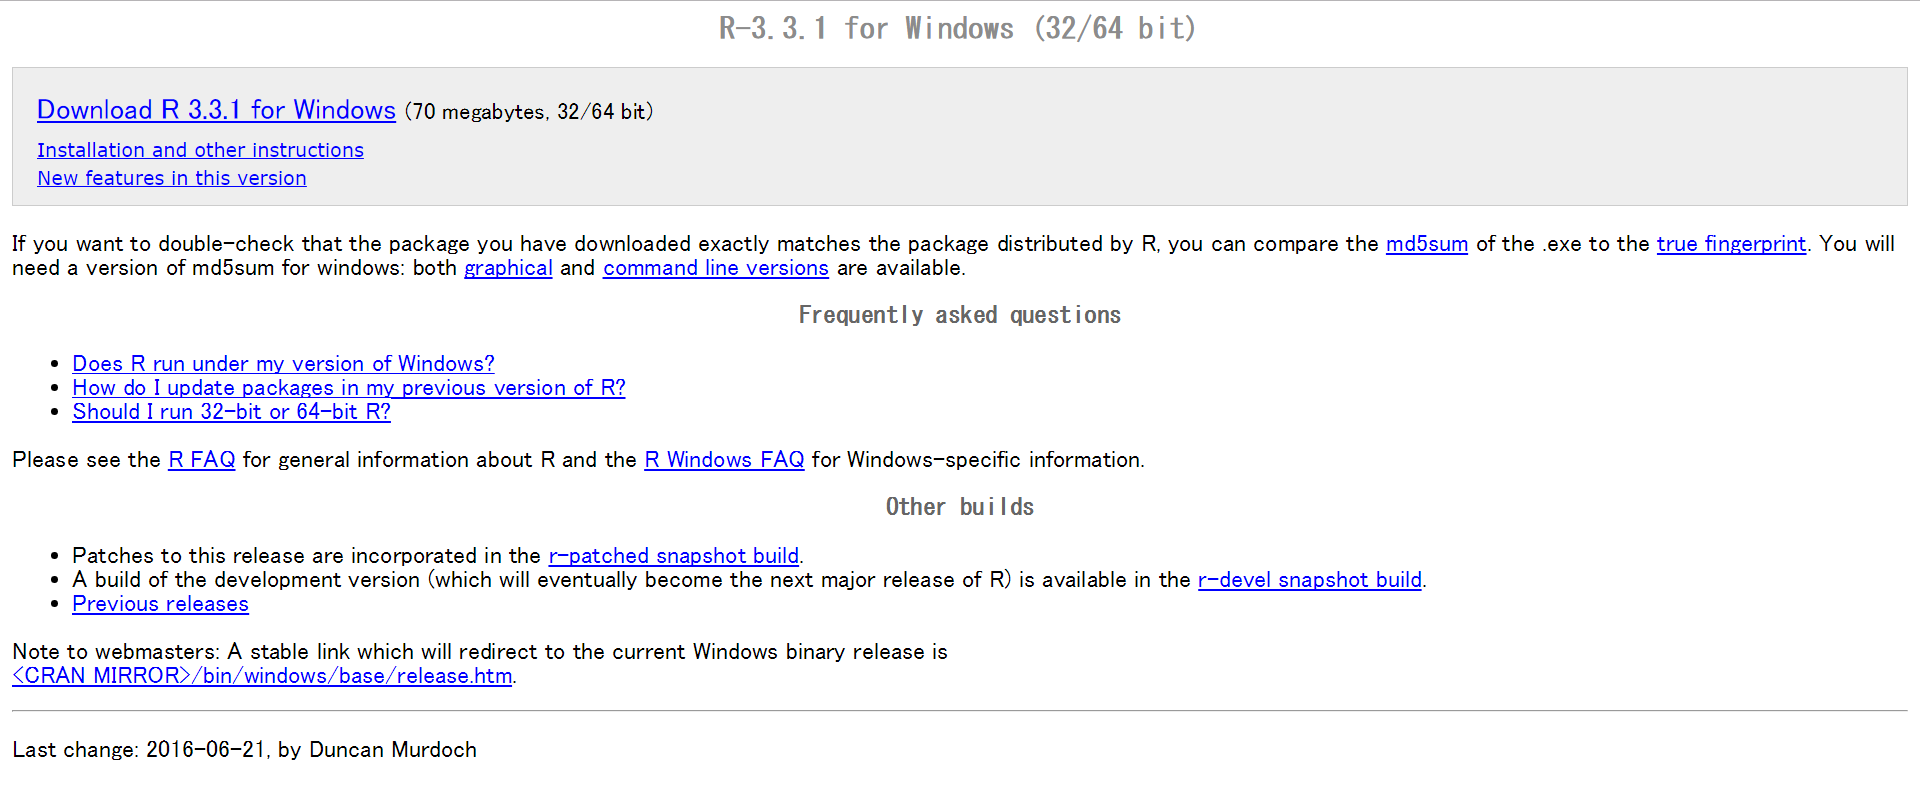
\includegraphics[width=13cm]{rinst2.png}
\caption{Download R 3.3.1 for Windowsをクリック}
\end{figure}

\newpage

インストーラーがダウンロードできたら起動しする.

確認し次へ
\begin{figure}[!htbp]
\centering 
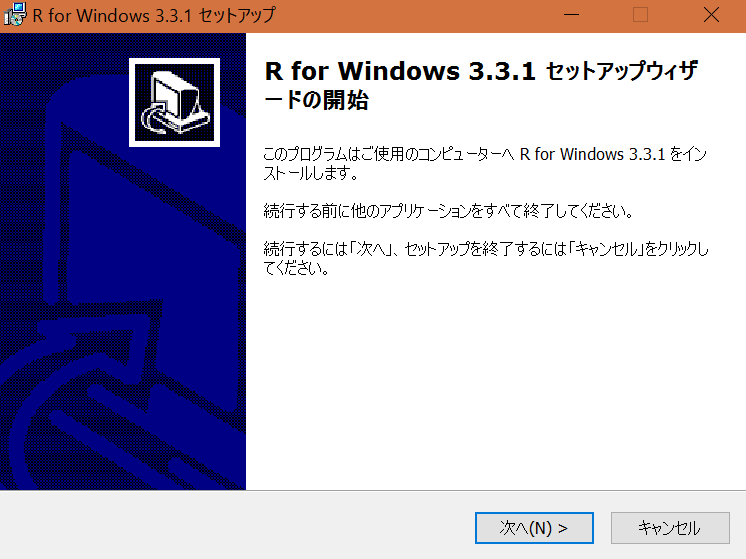
\includegraphics[width=13cm]{rinstall1.png}
\caption{1ページ目}
\end{figure}

\newpage
確認し次へ
\begin{figure}[!htbp]
\centering 
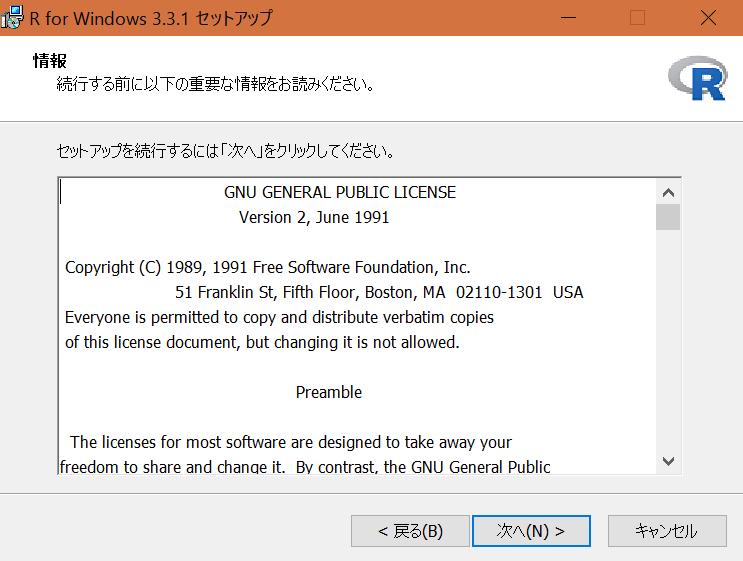
\includegraphics[width=13cm]{rinstall2.png}
\caption{2ページ目}
\end{figure}

\newpage

インストール先のディレクトリ変更する場合はここで変更.
\begin{figure}[!htbp]
\centering 
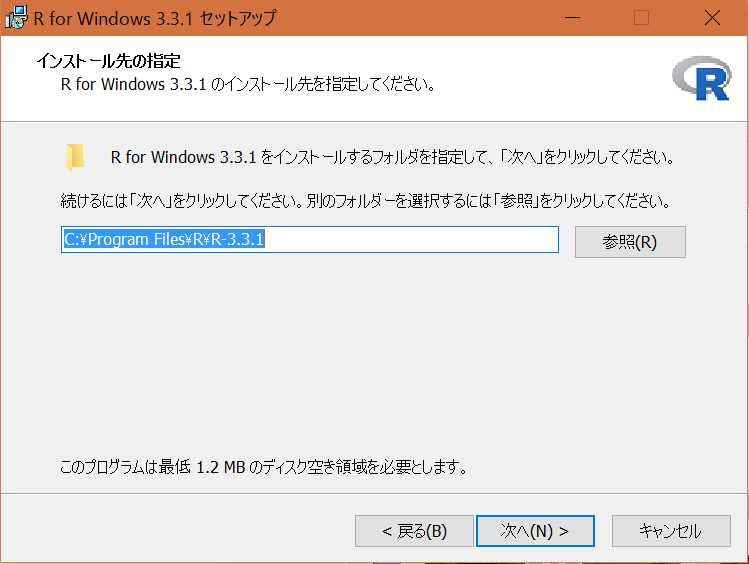
\includegraphics[width=13cm]{rinstall3.png}
\caption{3ページ目}
\end{figure}

\newpage

ここでWindowsが64bit版か32bit版かでインストールするものを決める.(デフォルトでは両方インストールされる.)

\begin{figure}[!htbp]
\centering 
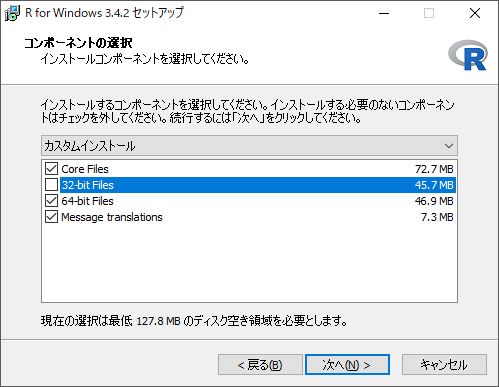
\includegraphics[width=13cm]{rinstall4.png}
\caption{4ページ目,32bit版か64bit版のチェックを外す}
\end{figure}

\newpage

起動時オプションをカスタマイズできるが,基本しなくても問題ない.

\begin{figure}[!htbp]
\centering 
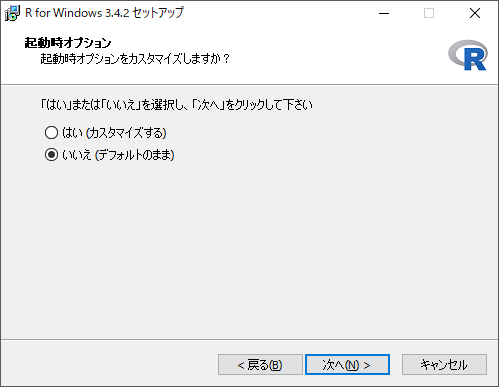
\includegraphics[width=13cm]{rinstall5.png}
\caption{5ページ目}
\end{figure}

\newpage

ここはそのままで構わない.

\begin{figure}[!htbp]
\centering 
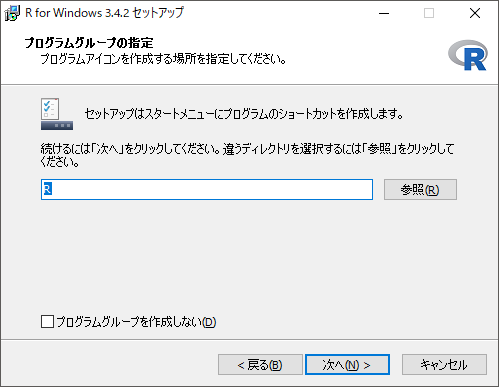
\includegraphics[width=13cm]{rinstall6.png}
\caption{6ページ目}
\end{figure}

\newpage

上の二つでショートカットアイコンやクイック起動アイコンを作成するか決める.下の2つチェックは入れておく.

\begin{figure}[!htbp]
\centering 
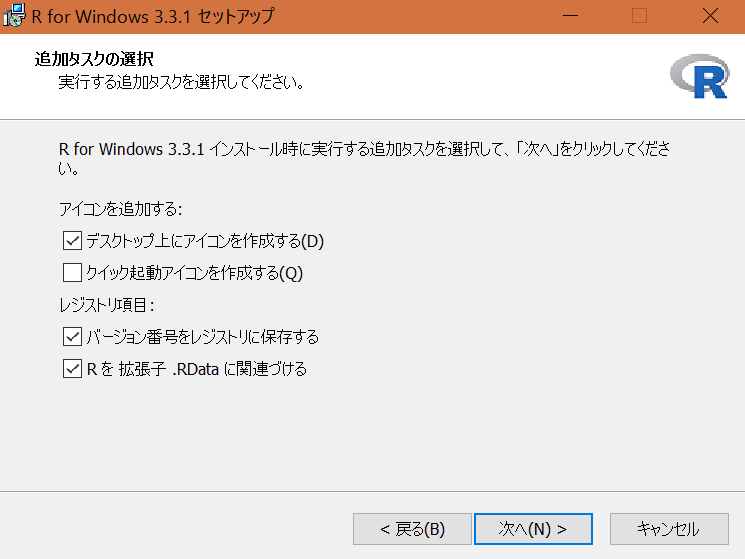
\includegraphics[width=13cm]{rinstall7.png}
\caption{7ページ目}
\end{figure}

\newpage

ゲージがマックスになれば完了.

\begin{figure}[!htbp]
\centering 
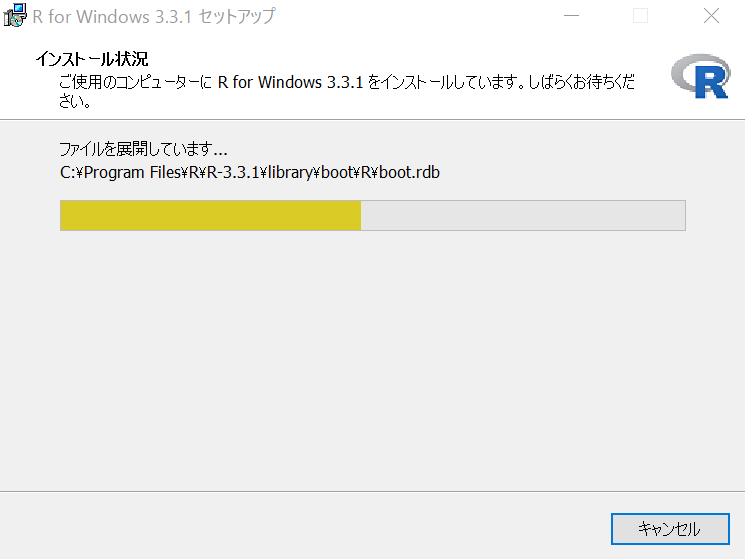
\includegraphics[width=13cm]{rinstall8.png}
\caption{8ページ目}
\end{figure}

\newpage
\subsubsection{Chocolateyを使ったインストール}



以下のコマンドでRをインストールする.\\

texttt{cinstl -y r.project}\\

デスクトップにRのショートカットが追加されていれば成功である.

\newpage

\subsection{ExcelとRのデータのやり取り}

\begin{figure}[!htbp]
\centering 
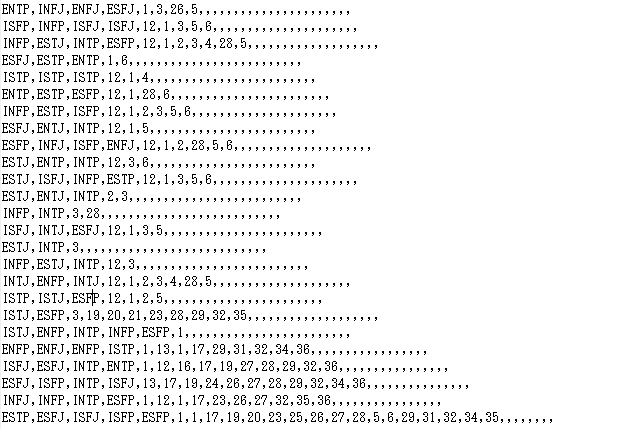
\includegraphics[width=13cm]{Acsv.png}
\caption{8ページ目}
\end{figure}



上記のようにグループごとにタイプ,発生したリスクを1行にしたデータをCSV形式で保存する.CSV形式は「,」区切りでデータを区切るファイル形式で,テキストファイルであるという特徴からアプリケーション間でデータをやり取りするときに使われることが多い.RとExcelとの間でやり取りする際にも便利で,本研究でもExcelで作成したデータはCSVファイルとして保存して使用する.また,本研究ではRによる作業ディレクトリをCドライブ直下に「cit」という名前で作成し,そのディレクトリ内に解析に使用するCSVファイル「メンバの性格と発生リスク.csv」を入れる.今回用いた解析方法はアソシエーション分析である.
\newpage

\subsection{使用したコード}

アソシエーション分析に使用したコードを記述する.\\

\begin{verbatim}

setwd('c:/cit')
install.packages('arules')
library(arules)

data <- read.transactions('メンバの性格と発生リスク.csv', sep = ',')
summary(data)

result <- apriori(data, parameter = list(support = 0.1, confidence = 0.5
, minlen = 3, maxlen = 5))

result
inspect(result[1:3])

clabels <- c("ENFJ","ENFP","ENTJ","ENTP","ESFJ","ESFP","ESTJ","ESTP","INFJ"
,"INFP","INTJ","INTP","ISFJ","ISFP","ISTJ","ISTP")

rlabels <- as.character(1:34)

rules <- subset(result, !(lhs %in% rlabels) & !(rhs %in% clabels))
rules
inspect(sort(rules, by = 'confidence'))

\end{verbatim}
\newpage
\subsection{今回用いたデータ}
今回用いたデータである.MBTIのタイプとグループ内で実際に起きたリスクを一行にまとめたものである.リスクにはあらかじめ数字を割り振り,データ化する際に数字を代入した.

データ一覧

%ここにMBTIのタイプとアンケートを貼る(学籍番号や名前は除く)
ISFP	ISTP	ISFP	ESFJ	ISFP	ESFP	6	7	9	11	3	13	14	16	17	20	21	22	23	24	25	27	28	29	30	31	32	33	34		

ISFP	ISFP	ESFP	ESFJ	ISFJ	7	14	17	25	27	30	33	34																		

ESFJ	ESFP	ISFP	ESFP	ESFJ	7	9	13	15	16	17	18	23	24	27	30	32	33													

ESFJ	ESFP	ISTJ	ISTJ	ISFP	11	3	14	16	17	21	23	30																		

ESTP	ESFJ	ISFJ	ISFP	ESFP	11	11	14	16	17	20	22	23	24	25	26	27	29	30	32	33										

ISTJ	ENFP	INTP	INFP	ESFP	11																									

ESFP	ESFJ	ISFJ	ISFP	ESFJ	11	4	7	8	11	14	16	17	18	21	22	23	24	31												

ESFJ	ISFP	INTP	ISFJ	7	14	16	21	23	24	27	30	32	34																	

ISTP	ENTP	INFP	ESTP	4	7	8	9	14	16	17	18	22	24	27	29	33														

ESTP	ESTJ	ESFP	ESFP	4	7	11	13	16	17	18	23	30	34																	

ENFP	ENFJ	ENFP	ISTP	11	7	11	14	27	29	30	32	34																		

INFJ	ISFP	ISFJ	ESTP	1	4	11	3	14	15	17	18	21	30	31	33															

ISFP	INFJ	ISTJ	ISTP	11	4	11	14	16	23	24	28																			

INFJ	INFP	INTP	ESFP	11	4	11	14	20	23	30	33	34																		

ISFJ	ESFJ	INTP	ENTP	11	4	13	14	16	24	27	30	34																		

ENTP	INFJ	ENFJ	ESFJ	11	3	23	25																							

ISFP	INFP	ISFJ	ISFJ	4	11	3	25	26																						

ESTJ	ISFJ	INFP	ESTP	4	11	3	25	26																						

INFP	ESTJ	INTP	ESFP	4	11	3	24	25																						

ESFP	INFJ	ISFP	ENFJ	4	11	24	25	26																						

ESFJ	ESTP	ENTP	11	26																										

INFP	ESTJ	INTP	4	3																										

ESTJ	ENTJ	INTP	3																											

ENTP	ESTP	ESFP	4	11	24	26																								

ESFJ	ISFJ	ESFP	11	4	7	8	11	14	16	17	18	21	22	23	24	31														

ENTJ	ISFP	ENFP	11	4	7	11	13	16	17	18	19	20	21	22	23	24	25	29	30	32	33									

INTP	INTP	ISFJ	1	2	5	14	16	18	23	24	28																			

ESTJ	ENTP	INTP	4	3	26																									

ESFJ	ENTJ	INTP	4	11	25																									

ISTP	ISTP	ISTP	4	11																										

ISFJ	INTJ	ESFJ	4	11	3	25																								

INFP	ESTP	ISFP	4	11	3	25	26																							

INTJ	ENFP	INTJ	4	11	3	24	25																							

ISTP	ISTJ	ESFP	4	11	25																									

ISTP	ENTJ	ISTP	1	6	11	3	13	14	24	25	28	30																		

ESTJ	INTP	3																												

INFJ	INTP	16	33																											

INFP	INTP	3	24																											

ISTJ	ESFP	3	16	17	18	20	24	27	30	33																				

INFP	ENFP	ENFP	ENFP	1	2	3	4	5	6	9	11	12	14	15	18	20	21	23	25	28	29	30								

ENTP	ISTJ	1	3	4	5	6	7	9	11	14	16	20	21	23	27	28	29	32	34											

INTP	ISTJ	ISFJ	ISFP	ESFJ	1	2	3	4	5	6	10	11	20	22	23	29	30	33												

ENFP	ISTJ	ESTP	ENFP	1	2	3	4	6	8	9	11	13	14	15	16	17	19	21	23	24	25	26	27	28	30	32	33	34		

ISFP	ESFJ	ISFJ	ESFJ	ISTP	1	2	3	4	5	6	7	8	9	10	11	13	14	16	17	18	20	21	22	23	24	27	28	29	32	33

ENTP	ESFP	ESTP	ISFJ	ESFP	1	4	5	6	11	14	16	20	24	28	34															

INTP	INTP	ISFP	1	5	6	10	13	14	17	18	23	24	33																	

INFP	ENTP	ENTP	ISTJ	ESFP	1	2	3	4	5	6	8	11	13	15	17	18	19	21	24	25	27	28	30	33						

ESFJ	ESFJ	ENFP	ENTJ	ISFP	1	2	4	5	6	7	11	13	14	20	22	24	25	27	33											

INTP	ESFJ	ENFP	ESFJ	1	4	5	6	11	12	14	22	23	24	25	26	27	28	30	33	34										

ENFJ	ISFP	ESTP	ESFP	1	2	3	4	5	6	9	10	11	12	13	14	16	17	18	20	21	22	23	24	25	27	28	29	30	31	34

ENTJ	ENFP	ISTP	ESFP	1	3	4	5	12	14	16	17	23	24	25	27	29	34													

ESFJ	INFP	ISFJ	1	3	4	5	6	8	9	10	11	13	14	16	18	20	21	23	24	25	27	28	32	34						

INTP	ISFJ	ESFP	ISFP	ENTP	1	2	3	4	5	6	8	11	12	13	14	16	18	27	29	32	33	34								

INFJ	ISTP	ENFJ	INFJ	1	4	5	6	10	11	14	17	20	24	29	34															

ESFJ	INFP	ENFP	1	3	5	6	8	9	10	11	16	20	22	25																

ESFJ	ESFP	ISTP	ISFP	ENFP	1	3	4	5	6	7	8	9	11	13	14	16	17	18	20	23	24	25	27	30	34					

ESFJ	ESTP	ESFP	ESFJ	1	2	3	4	5	6	7	11	12	13	14	15	27	30	31	32	33	34									

ESFJ	INFJ	ESFJ	ESFJ	1	2	4	5	6	7	8	9	11	13	14	16	17	18	20	23	24	33	34								

ESTP	ISTP	INTP	1	4	5	6	10	11	14	15	16	20	21	25	27	28														

INTP	ESFJ	ISTP	ENTJ	ENTJ	5	20	25																							

ISFJ	ESTP	ISFJ	1	2	3	4	5	6	12	16	18	20	25	27	28															

ISFJ	ISFP	1	3	4	5	6	11	14	16	20	24	27	32																	

ESTJ	ESFP	ENTP	ESFP	1	2	3	4	7	9	14	16	23	24	27	29	32	34													

ISFP	ISFP	ENTP	ESTJ	1	2	3	7	8	11	14	16	17	18	23	24	27	30	31	32	33	34									

ENTJ	INTP	ISFJ	ISFP	1	3	4	5	7	11	12	13	14	16	20	22	24	25	27	29	32	33	34								

ESTP	INTP	ISTP	4	5	14	16	20	33	34																					

ENFP	ENTJ	ENTP	ISTP	1	4	5	6	7	8	9	11	12	14	18	22	24	25	27	28	29	31	32	33	34						

ENFP	ESTJ	ISFJ	1	4	5	6	7	11	12	14	16	17	18	27	30	33	34													

ESFJ	INTP	ISTJ	1	2	3	4	5	6	12	13	14	16	17	21	24	25	27	28	29	30	32	33	34							

ESFJ	ESFJ	ESFJ	INFP	1	3	4	5	6	9	11	12	13	14	16	17	18	20	22	23	24	25									

ENFJ	ESFJ	ESTP	ISTP	1	2	3	4	5	6	7	8	9	11	13	14	15	16	17	18	20	21	22	23	24	25	28	29	30	34	

ESFJ	ESTP	ISFJ	1	2	3	4	5	6	11	12	14	16	20	23	24	27	28	29	32											

ESFJ	INTP	ISFP	2	3	4	12	14	30																						

\newpage

\subsection{リスク一覧}
1	計画の見通しが甘かった.

2	想定外のアクシデントが起きた.

3	スケジュールに遅れが出た.

4	技術的に困難なことは他人に任せた.

5	仕事量が偏っていた.

6	分担が適切ではなかった.

7	いい成績を取るという意欲はなかった.

8	メンバーが何をしたのか把握していない.

9	リーダーの指示はすべて把握していない.

10	えこひいきがあった.

11	作業の割り振りは妥当ではなかった.

12	自分の作業を決められた通りの期日に遅れた.

13	進んで作業に取り組めなかった.

14	単位を取れればいいやという気持ちはあった.

15	メンバーと前より仲が悪くなった.

16	毎週の連絡を忘れた.

17	成果物や作業指示の確認を怠った.

18	進捗を把握していない.

19	間違って同じ作業をしてしまった.

20	作業量が自分だけ多かった.

21	リーダーの指示がわかりにくかった.

22	意見を聞いてもらえず話し合いにならないことがあった.

23	話し合いで無言が続いた.

24	話し合いの場で進んで発言できなかった.

25	情報共有は問題があった.

26	チーム内で諍いが起きた.

27	講義を休んだ.

28	リーダーの指示は的確ではなかった.

29	やらされているようであった.

30	提出物に関係するものに不備があった.

31	途中退席した.

32	無断欠席した.

33	雑談が多かった.

34	講義に関係ないことをしていた.

\section{アソシエーション分析の抽出結果}
アソシエーション分析の結果である.
左からどのタイプがいるとき,どのリスクが起きるか,発生率,確信度となっている.lift値とは発生率と確信度を掛けた値である.

%上記のデータから得られたルールを貼る
      lhs                      rhs  support    confidence lift      count


[1]   {ENFJ,INFJ}           => {11} 0.04109589 1.0000000  1.3773585  3   

[2]   {INFJ,ISFP}           => {4}  0.04109589 1.0000000  1.4038462  3   

[3]   {INFJ,ISFP}           => {11} 0.04109589 1.0000000  1.3773585  3   

[4]   {ENFJ,ISTP}           => {29} 0.04109589 1.0000000  3.8421053  3   

[5]   {ENFJ,ISTP}           => {34} 0.04109589 1.0000000  2.7037037  3   

[6]   {ENFJ,ISTP}           => {14} 0.04109589 1.0000000  1.6590909  3   

[7]   {ENFJ,ISTP}           => {11} 0.04109589 1.0000000  1.3773585  3   

[8]   {ESTJ,INFP}           => {3}  0.04109589 1.0000000  1.8250000  3   

[9]   {ESTJ,INFP}           => {4}  0.04109589 1.0000000  1.4038462  3   

[10]  {ENTP,ESTJ}           => {3}  0.04109589 1.0000000  1.8250000  3   

[11]  {ESTJ,INTP}           => {3}  0.06849315 1.0000000  1.8250000  5   

[12]  {ESFP,ESTJ}           => {4}  0.04109589 1.0000000  1.4038462  3   

[13]  {ENFP,ENTJ}           => {25} 0.05479452 1.0000000  2.2121212  4   

[14]  {ENFP,ENTJ}           => {24} 0.05479452 1.0000000  1.8250000  4   

[15]  {ENFP,ENTJ}           => {4}  0.05479452 1.0000000  1.4038462  4   

[16]  {ENTJ,ISTP}           => {25} 0.05479452 1.0000000  2.2121212  4   

[17]  {ENTJ,ISFP}           => {22} 0.04109589 1.0000000  4.5625000  3   

[18]  {ENTJ,ISFP}           => {7}  0.04109589 1.0000000  3.3181818  3   

[19]  {ENTJ,ISFP}           => {13} 0.04109589 1.0000000  3.4761905  3   

[20]  {ENTJ,ISFP}           => {33} 0.04109589 1.0000000  2.8076923  3   

[21]  {ENTJ,ISFP}           => {20} 0.04109589 1.0000000  2.8076923  3   

[22]  {ENTJ,ISFP}           => {25} 0.04109589 1.0000000  2.2121212  3   

[23]  {ENTJ,ISFP}           => {24} 0.04109589 1.0000000  1.8250000  3   

[24]  {ENTJ,ISFP}           => {4}  0.04109589 1.0000000  1.4038462  3   

[25]  {ENTJ,ISFP}           => {11} 0.04109589 1.0000000  1.3773585  3   

[26]  {ENTJ,ESFJ}           => {25} 0.04109589 1.0000000  2.2121212  3   

[27]  {ISFP,ISTJ}           => {23} 0.04109589 1.0000000  2.4333333  3   

[28]  {ISFP,ISTJ}           => {11} 0.04109589 1.0000000  1.3773585  3   

[29]  {ESFJ,ISTJ}           => {30} 0.04109589 1.0000000  2.7037037  3   

[30]  {ESFJ,ISTJ}           => {3}  0.04109589 1.0000000  1.8250000  3   

[31]  {ENFP,INFP}           => {11} 0.04109589 1.0000000  1.3773585  3   

[32]  {ESTP,INFP}           => {4}  0.04109589 1.0000000  1.4038462  3   

[33]  {INFP,ISFJ}           => {25} 0.04109589 1.0000000  2.2121212  3   

[34]  {INFP,ISFJ}           => {3}  0.04109589 1.0000000  1.8250000  3   

[35]  {INFP,ISFJ}           => {4}  0.04109589 1.0000000  1.4038462  3   

[36]  {INFP,ISFJ}           => {11} 0.04109589 1.0000000  1.3773585  3   

[37]  {ESFP,INFP}           => {11} 0.05479452 1.0000000  1.3773585  4   

[38]  {ESFJ,INFP}           => {9}  0.04109589 1.0000000  4.5625000  3   

[39]  {ESFJ,INFP}           => {20} 0.04109589 1.0000000  2.8076923  3   

[40]  {ESFJ,INFP}           => {25} 0.04109589 1.0000000  2.2121212  3   

[41]  {ESFJ,INFP}           => {6}  0.04109589 1.0000000  2.5172414  3   

[42]  {ESFJ,INFP}           => {5}  0.04109589 1.0000000  2.3548387  3   

[43]  {ESFJ,INFP}           => {3}  0.04109589 1.0000000  1.8250000  3   

[44]  {ESFJ,INFP}           => {1}  0.04109589 1.0000000  2.1470588  3   

[45]  {ESFJ,INFP}           => {16} 0.04109589 1.0000000  1.9210526  3   

[46]  {ESFJ,INFP}           => {11} 0.04109589 1.0000000  1.3773585  3   

[47]  {ENTP,INTP}           => {4}  0.04109589 1.0000000  1.4038462  3   

[48]  {ENTP,ISFJ}           => {34} 0.04109589 1.0000000  2.7037037  3   

[49]  {ENTP,ISFJ}           => {16} 0.04109589 1.0000000  1.9210526  3   

[50]  {ENTP,ISFJ}           => {14} 0.04109589 1.0000000  1.6590909  3   

[51]  {ENTP,ISFJ}           => {4}  0.04109589 1.0000000  1.4038462  3   

[52]  {ENTP,ISFJ}           => {11} 0.04109589 1.0000000  1.3773585  3   

[53]  {ENTP,ESFP}           => {4}  0.06849315 1.0000000  1.4038462  5   

[54]  {ENTP,ESFJ}           => {11} 0.04109589 1.0000000  1.3773585  3   

[55]  {ENFP,ISTP}           => {34} 0.05479452 1.0000000  2.7037037  4   

[56]  {ENFP,ISTP}           => {27} 0.05479452 1.0000000  2.3548387  4   

[57]  {ENFP,ISTP}           => {14} 0.05479452 1.0000000  1.6590909  4   

[58]  {ENFP,ISFP}           => {7}  0.04109589 1.0000000  3.3181818  3   

[59]  {ENFP,ISFP}           => {13} 0.04109589 1.0000000  3.4761905  3   

[60]  {ENFP,ISFP}           => {20} 0.04109589 1.0000000  2.8076923  3   

[61]  {ENFP,ISFP}           => {25} 0.04109589 1.0000000  2.2121212  3   

[62]  {ENFP,ISFP}           => {24} 0.04109589 1.0000000  1.8250000  3   

[63]  {ENFP,ISFP}           => {4}  0.04109589 1.0000000  1.4038462  3   

[64]  {ENFP,ISFP}           => {11} 0.04109589 1.0000000  1.3773585  3   

[65]  {ENFP,ESFJ}           => {25} 0.05479452 1.0000000  2.2121212  4   

[66]  {ENFP,ESFJ}           => {6}  0.05479452 1.0000000  2.5172414  4   

[67]  {ENFP,ESFJ}           => {5}  0.05479452 1.0000000  2.3548387  4   

[68]  {ENFP,ESFJ}           => {1}  0.05479452 1.0000000  2.1470588  4   

[69]  {ENFP,ESFJ}           => {11} 0.05479452 1.0000000  1.3773585  4   

[70]  {INTP,ISTP}           => {20} 0.04109589 1.0000000  2.8076923  3   

[71]  {INTP,ISTP}           => {5}  0.04109589 1.0000000  2.3548387  3   

[72]  {ESFP,INTP}           => {11} 0.05479452 1.0000000  1.3773585  4   

[73]  {ESTP,ISTP}           => {16} 0.05479452 1.0000000  1.9210526  4   

[74]  {ESTP,ISTP}           => {14} 0.05479452 1.0000000  1.6590909  4   

[75]  {ESTP,ISTP}           => {4}  0.05479452 1.0000000  1.4038462  4   

[76]  {ESFP,ISTP}           => {25} 0.05479452 1.0000000  2.2121212  4   

[77]  {ISFP,ISTP}           => {23} 0.05479452 1.0000000  2.4333333  4   

[78]  {ISFP,ISTP}           => {16} 0.05479452 1.0000000  1.9210526  4   

[79]  {ISFP,ISTP}           => {24} 0.05479452 1.0000000  1.8250000  4   

[80]  {ISFP,ISTP}           => {14} 0.05479452 1.0000000  1.6590909  4   

[81]  {ISFP,ISTP}           => {11} 0.05479452 1.0000000  1.3773585  4   

[82]  {ESFJ,ISTP}           => {20} 0.06849315 1.0000000  2.8076923  5   

[83]  {ESFP,ESTP}           => {11} 0.08219178 1.0000000  1.3773585  6   

[84]  {ESTP,ISFP}           => {11} 0.05479452 1.0000000  1.3773585  4   

[85]  {ESFJ,ESTP}           => {11} 0.06849315 1.0000000  1.3773585  5   

[86]  {ESFP,ISFJ}           => {14} 0.08219178 1.0000000  1.6590909  6   

[87]  {ESFP,INFP,INTP}      => {11} 0.04109589 1.0000000  1.3773585  3   

[88]  {ESFJ,INTP,ISFJ}      => {30} 0.04109589 1.0000000  2.7037037  3   

[89]  {ESFJ,INTP,ISFP}      => {30} 0.04109589 1.0000000  2.7037037  3   

[90]  {ESFJ,ISFP,ISTP}      => {9}  0.04109589 1.0000000  4.5625000  3   

[91]  {ESFJ,ISFP,ISTP}      => {7}  0.04109589 1.0000000  3.3181818  3   

[92]  {ESFJ,ISFP,ISTP}      => {13} 0.04109589 1.0000000  3.4761905  3   

[93]  {ESFJ,ISFP,ISTP}      => {20} 0.04109589 1.0000000  2.8076923  3   

[94]  {ESFJ,ISFP,ISTP}      => {17} 0.04109589 1.0000000  2.8076923  3   

[95]  {ESFJ,ISFP,ISTP}      => {23} 0.04109589 1.0000000  2.4333333  3   

[96]  {ESFJ,ISFP,ISTP}      => {6}  0.04109589 1.0000000  2.5172414  3   

[97]  {ESFJ,ISFP,ISTP}      => {27} 0.04109589 1.0000000  2.3548387  3   

[98]  {ESFJ,ISFP,ISTP}      => {3}  0.04109589 1.0000000  1.8250000  3   

[99]  {ESFJ,ISFP,ISTP}      => {16} 0.04109589 1.0000000  1.9210526  3   

[100] {ESFJ,ISFP,ISTP}      => {24} 0.04109589 1.0000000  1.8250000  3   

[101] {ESFJ,ISFP,ISTP}      => {14} 0.04109589 1.0000000  1.6590909  3   

[102] {ESFJ,ISFP,ISTP}      => {11} 0.04109589 1.0000000  1.3773585  3   

[103] {ESFP,ISFJ,ISFP}      => {14} 0.05479452 1.0000000  1.6590909  4   

[104] {ESFJ,ESFP,ISFJ}      => {17} 0.05479452 1.0000000  2.8076923  4   

[105] {ESFJ,ESFP,ISFJ}      => {14} 0.05479452 1.0000000  1.6590909  4   

[106] {ESFJ,ESFP,ISFP}      => {17} 0.09589041 1.0000000  2.8076923  7   

[107] {ESFJ,ESFP,ISFJ,ISFP} => {17} 0.04109589 1.0000000  2.8076923  3   

[108] {ESFJ,ESFP,ISFJ,ISFP} => {14} 0.04109589 1.0000000  1.6590909  3   

[109] {ESFJ,ESFP}           => {17} 0.10958904 0.8888889  2.4957265  8   

[110] {ESFJ,ESFP}           => {14} 0.10958904 0.8888889  1.4747475  8   

[111] {ESFJ,ESFP,ISFP}      => {30} 0.08219178 0.8571429  2.3174603  6   

[112] {ESFJ,ESFP,ISFP}      => {23} 0.08219178 0.8571429  2.0857143  6   

[113] {ESFJ,ESFP,ISFP}      => {16} 0.08219178 0.8571429  1.6466165  6   

[114] {ESFJ,ESFP,ISFP}      => {14} 0.08219178 0.8571429  1.4220779  6   

[115] {INTP,ISFJ}           => {16} 0.06849315 0.8333333  1.6008772  5   

[116] {INTP,ISFJ}           => {14} 0.06849315 0.8333333  1.3825758  5   

[117] {INTP,ISFP}           => {14} 0.06849315 0.8333333  1.3825758  5   

[118] {ESTP,ISFJ}           => {4}  0.06849315 0.8333333  1.1698718  5   

[119] {ESTP,ISFJ}           => {11} 0.06849315 0.8333333  1.1477987  5   

[120] {ESFP,ESTP}           => {4}  0.06849315 0.8333333  1.1698718  5   

[121] {ESFP,ISFJ}           => {16} 0.06849315 0.8333333  1.6008772  5   

[122] {ESFP,ISFJ}           => {11} 0.06849315 0.8333333  1.1477987  5   

[123] {ESFJ,ISFP}           => {14} 0.13698630 0.8333333  1.3825758 10   

[124] {ESFJ,ISFJ,ISFP}      => {23} 0.06849315 0.8333333  2.0277778  5   

[125] {ESFJ,ISFJ,ISFP}      => {14} 0.06849315 0.8333333  1.3825758  5   

[126] {ISFJ,ISFP}           => {14} 0.12328767 0.8181818  1.3574380  9   

[127] {ISFJ,ISFP}           => {11} 0.12328767 0.8181818  1.1269297  9   

[128] {ESFJ,ISFJ}           => {14} 0.12328767 0.8181818  1.3574380  9   

[129] {ESFJ,ISFJ}           => {11} 0.12328767 0.8181818  1.1269297  9   

[130] {ESFP,ISTJ}           => {11} 0.05479452 0.8000000  1.1018868  4   

[131] {ENTP,ESFP}           => {1}  0.05479452 0.8000000  1.7176471  4   

[132] {ENTP,ESFP}           => {24} 0.05479452 0.8000000  1.4600000  4   

[133] {ENTP,ESFP}           => {11} 0.05479452 0.8000000  1.1018868  4   

[134] {ESFJ,ISTP}           => {9}  0.05479452 0.8000000  3.6500000  4   

[135] {ESFJ,ISTP}           => {7}  0.05479452 0.8000000  2.6545455  4   

[136] {ESFJ,ISTP}           => {13} 0.05479452 0.8000000  2.7809524  4   

[137] {ESFJ,ISTP}           => {17} 0.05479452 0.8000000  2.2461538  4   

[138] {ESFJ,ISTP}           => {25} 0.05479452 0.8000000  1.7696970  4   

[139] {ESFJ,ISTP}           => {23} 0.05479452 0.8000000  1.9466667  4   

[140] {ESFJ,ISTP}           => {6}  0.05479452 0.8000000  2.0137931  4   

[141] {ESFJ,ISTP}           => {5}  0.05479452 0.8000000  1.8838710  4   

[142] {ESFJ,ISTP}           => {3}  0.05479452 0.8000000  1.4600000  4   

[143] {ESFJ,ISTP}           => {16} 0.05479452 0.8000000  1.5368421  4   

[144] {ESFJ,ISTP}           => {24} 0.05479452 0.8000000  1.4600000  4   

[145] {ESFJ,ISTP}           => {14} 0.05479452 0.8000000  1.3272727  4   

[146] {ESFJ,ISTP}           => {11} 0.05479452 0.8000000  1.1018868  4   

[147] {ESFJ,ESTP}           => {14} 0.05479452 0.8000000  1.3272727  4   

[148] {ESFP,ISFP}           => {17} 0.10958904 0.8000000  2.2461538  8   

[149] {ESFP,ISFP}           => {16} 0.10958904 0.8000000  1.5368421  8   

[150] {ESFP,ISFP}           => {14} 0.10958904 0.8000000  1.3272727  8   

[151] {ESFP,ISFP}           => {11} 0.10958904 0.8000000  1.1018868  8   

[152] {ESFJ,ESFP}           => {7}  0.09589041 0.7777778  2.5808081  7   

[153] {ESFJ,ESFP}           => {30} 0.09589041 0.7777778  2.1028807  7   

[154] {ESFJ,ESFP}           => {23} 0.09589041 0.7777778  1.8925926  7   

[155] {ESFJ,ESFP}           => {16} 0.09589041 0.7777778  1.4941520  7   

[156] {ESFJ,ESFP}           => {11} 0.09589041 0.7777778  1.0712788  7   

[157] {ENFP,ENTJ}           => {22} 0.04109589 0.7500000  3.4218750  3   

[158] {ENFP,ENTJ}           => {29} 0.04109589 0.7500000  2.8815789  3   

[159] {ENFP,ENTJ}           => {7}  0.04109589 0.7500000  2.4886364  3   

[160] {ENFP,ENTJ}           => {33} 0.04109589 0.7500000  2.1057692  3   

[161] {ENFP,ENTJ}           => {5}  0.04109589 0.7500000  1.7661290  3   

[162] {ENFP,ENTJ}           => {27} 0.04109589 0.7500000  1.7661290  3   

[163] {ENFP,ENTJ}           => {1}  0.04109589 0.7500000  1.6102941  3   

[164] {ENFP,ENTJ}           => {14} 0.04109589 0.7500000  1.2443182  3   

[165] {ENFP,ENTJ}           => {11} 0.04109589 0.7500000  1.0330189  3   

[166] {ENTJ,INTP}           => {25} 0.04109589 0.7500000  1.6590909  3   

[167] {ENTJ,ISTP}           => {5}  0.04109589 0.7500000  1.7661290  3   

[168] {ENTJ,ISTP}           => {1}  0.04109589 0.7500000  1.6102941  3   

[169] {ENTJ,ISTP}           => {24} 0.04109589 0.7500000  1.3687500  3   

[170] {ENTJ,ISTP}           => {14} 0.04109589 0.7500000  1.2443182  3   

[171] {ESFP,INFP}           => {4}  0.04109589 0.7500000  1.0528846  3   

[172] {ENTP,ESTP}           => {24} 0.04109589 0.7500000  1.3687500  3   

[173] {ENTP,ESTP}           => {4}  0.04109589 0.7500000  1.0528846  3   

[174] {ENTP,ESTP}           => {11} 0.04109589 0.7500000  1.0330189  3   

[175] {ENFP,ISTP}           => {29} 0.04109589 0.7500000  2.8815789  3   

[176] {ENFP,ISTP}           => {7}  0.04109589 0.7500000  2.4886364  3   

[177] {ENFP,ISTP}           => {25} 0.04109589 0.7500000  1.6590909  3   

[178] {ENFP,ISTP}           => {5}  0.04109589 0.7500000  1.7661290  3   

[179] {ENFP,ISTP}           => {1}  0.04109589 0.7500000  1.6102941  3   

[180] {ENFP,ISTP}           => {24} 0.04109589 0.7500000  1.3687500  3   

[181] {ENFP,ISTP}           => {4}  0.04109589 0.7500000  1.0528846  3   

[182] {ENFP,ISTP}           => {11} 0.04109589 0.7500000  1.0330189  3   

[183] {ENFP,ESFJ}           => {22} 0.04109589 0.7500000  3.4218750  3   

[184] {ENFP,ESFJ}           => {20} 0.04109589 0.7500000  2.1057692  3   

[185] {ENFP,ESFJ}           => {27} 0.04109589 0.7500000  1.7661290  3   

[186] {ENFP,ESFJ}           => {24} 0.04109589 0.7500000  1.3687500  3   

[187] {ENFP,ESFJ}           => {14} 0.04109589 0.7500000  1.2443182  3   

[188] {ENFP,ESFJ}           => {4}  0.04109589 0.7500000  1.0528846  3   

[189] {ESFP,INTP}           => {4}  0.04109589 0.7500000  1.0528846  3   

[190] {ESFJ,INTP}           => {30} 0.08219178 0.7500000  2.0277778  6   

[191] {ESFJ,INTP}           => {4}  0.08219178 0.7500000  1.0528846  6   

[192] {ESTP,ISTP}           => {20} 0.04109589 0.7500000  2.1057692  3   

[193] {ESTP,ISTP}           => {5}  0.04109589 0.7500000  1.7661290  3   

[194] {ESFP,ISTP}           => {17} 0.04109589 0.7500000  2.1057692  3   

[195] {ESFP,ISTP}           => {34} 0.04109589 0.7500000  2.0277778  3   

[196] {ESFP,ISTP}           => {23} 0.04109589 0.7500000  1.8250000  3   

[197] {ESFP,ISTP}           => {27} 0.04109589 0.7500000  1.7661290  3   

[198] {ESFP,ISTP}           => {3}  0.04109589 0.7500000  1.3687500  3   

[199] {ESFP,ISTP}           => {16} 0.04109589 0.7500000  1.4407895  3   

[200] {ESFP,ISTP}           => {24} 0.04109589 0.7500000  1.3687500  3   

[201] {ESFP,ISTP}           => {14} 0.04109589 0.7500000  1.2443182  3   

[202] {ESFP,ISTP}           => {4}  0.04109589 0.7500000  1.0528846  3   

[203] {ESFP,ISTP}           => {11} 0.04109589 0.7500000  1.0330189  3   

[204] {ISFP,ISTP}           => {9}  0.04109589 0.7500000  3.4218750  3   

[205] {ISFP,ISTP}           => {28} 0.04109589 0.7500000  2.8815789  3   

[206] {ISFP,ISTP}           => {7}  0.04109589 0.7500000  2.4886364  3   

[207] {ISFP,ISTP}           => {13} 0.04109589 0.7500000  2.6071429  3   

[208] {ISFP,ISTP}           => {20} 0.04109589 0.7500000  2.1057692  3   

[209] {ISFP,ISTP}           => {17} 0.04109589 0.7500000  2.1057692  3   

[210] {ISFP,ISTP}           => {6}  0.04109589 0.7500000  1.8879310  3   

[211] {ISFP,ISTP}           => {27} 0.04109589 0.7500000  1.7661290  3   

[212] {ISFP,ISTP}           => {3}  0.04109589 0.7500000  1.3687500  3   

[213] {ISFP,ISTP}           => {4}  0.04109589 0.7500000  1.0528846  3   

[214] {ESTP,ISFP}           => {30} 0.04109589 0.7500000  2.0277778  3   

[215] {ESTP,ISFP}           => {17} 0.04109589 0.7500000  2.1057692  3   

[216] {ESTP,ISFP}           => {25} 0.04109589 0.7500000  1.6590909  3   

[217] {ESTP,ISFP}           => {3}  0.04109589 0.7500000  1.3687500  3   

[218] {ESTP,ISFP}           => {14} 0.04109589 0.7500000  1.2443182  3   

[219] {ESTP,ISFP}           => {4}  0.04109589 0.7500000  1.0528846  3   

[220] {ESFJ,ISFP}           => {30} 0.12328767 0.7500000  2.0277778  9   

[221] {ESFJ,ISFP}           => {23} 0.12328767 0.7500000  1.8250000  9   

[222] {INTP,ISFJ,ISFP}      => {32} 0.04109589 0.7500000  2.8815789  3   

[223] {INTP,ISFJ,ISFP}      => {29} 0.04109589 0.7500000  2.8815789  3   

[224] {INTP,ISFJ,ISFP}      => {33} 0.04109589 0.7500000  2.1057692  3   

[225] {INTP,ISFJ,ISFP}      => {34} 0.04109589 0.7500000  2.0277778  3   

[226] {INTP,ISFJ,ISFP}      => {5}  0.04109589 0.7500000  1.7661290  3   

[227] {INTP,ISFJ,ISFP}      => {27} 0.04109589 0.7500000  1.7661290  3   

[228] {INTP,ISFJ,ISFP}      => {3}  0.04109589 0.7500000  1.3687500  3   

[229] {INTP,ISFJ,ISFP}      => {1}  0.04109589 0.7500000  1.6102941  3   

[230] {INTP,ISFJ,ISFP}      => {16} 0.04109589 0.7500000  1.4407895  3   

[231] {INTP,ISFJ,ISFP}      => {14} 0.04109589 0.7500000  1.2443182  3   

[232] {INTP,ISFJ,ISFP}      => {4}  0.04109589 0.7500000  1.0528846  3   

[233] {INTP,ISFJ,ISFP}      => {11} 0.04109589 0.7500000  1.0330189  3   

[234] {ESFJ,ESFP,ISFJ}      => {22} 0.04109589 0.7500000  3.4218750  3   

[235] {ESFP,ISFJ,ISFP}      => {33} 0.04109589 0.7500000  2.1057692  3   

[236] {ESFP,ISFJ,ISFP}      => {17} 0.04109589 0.7500000  2.1057692  3   

[237] {ESFP,ISFJ,ISFP}      => {27} 0.04109589 0.7500000  1.7661290  3   

[238] {ESFP,ISFJ,ISFP}      => {16} 0.04109589 0.7500000  1.4407895  3   

[239] {ESFP,ISFJ,ISFP}      => {11} 0.04109589 0.7500000  1.0330189  3   

[240] {ESFJ,ESFP,ISFJ}      => {7}  0.04109589 0.7500000  2.4886364  3   

[241] {ESFJ,ESFP,ISFJ}      => {23} 0.04109589 0.7500000  1.8250000  3   

[242] {ESFJ,ESFP,ISFJ}      => {16} 0.04109589 0.7500000  1.4407895  3   

[243] {ESFJ,ESFP,ISFJ}      => {24} 0.04109589 0.7500000  1.3687500  3   

[244] {ESFJ,ESFP,ISFJ}      => {11} 0.04109589 0.7500000  1.0330189  3   

[245] {ISFJ,ISFP}           => {4}  0.10958904 0.7272727  1.0209790  8   

[246] {ESFJ,ISFJ}           => {23} 0.10958904 0.7272727  1.7696970  8   

[247] {ESFJ,ISFJ}           => {16} 0.10958904 0.7272727  1.3971292  8   

[248] {ESFJ,ISFJ}           => {24} 0.10958904 0.7272727  1.3272727  8   

[249] {ESFJ,ISFJ}           => {4}  0.10958904 0.7272727  1.0209790  8   

[250] {ESFJ,ESFP,ISFP}      => {7}  0.06849315 0.7142857  2.3701299  5   

[251] {ESFJ,ESFP,ISFP}      => {27} 0.06849315 0.7142857  1.6820276  5   

[252] {ESFJ,ESFP,ISFP}      => {24} 0.06849315 0.7142857  1.3035714  5   

[253] {ESFJ,ESFP,ISFP}      => {11} 0.06849315 0.7142857  0.9838275  5   

[254] {ESFP,ISFP}           => {30} 0.09589041 0.7000000  1.8925926  7   

[255] {ESFP,ISFP}           => {23} 0.09589041 0.7000000  1.7033333  7   

[256] {ESFP,ISFP}           => {27} 0.09589041 0.7000000  1.6483871  7   

[257] {ESFP,ISFP}           => {24} 0.09589041 0.7000000  1.2775000  7   

[258] {INTP,ISFJ}           => {34} 0.05479452 0.6666667  1.8024691  4   

[259] {INTP,ISFJ}           => {5}  0.05479452 0.6666667  1.5698925  4   

[260] {INTP,ISFJ}           => {27} 0.05479452 0.6666667  1.5698925  4   

[261] {INTP,ISFJ}           => {1}  0.05479452 0.6666667  1.4313725  4   

[262] {INTP,ISFJ}           => {24} 0.05479452 0.6666667  1.2166667  4   

[263] {INTP,ISFJ}           => {4}  0.05479452 0.6666667  0.9358974  4   

[264] {INTP,ISFJ}           => {11} 0.05479452 0.6666667  0.9182390  4   

[265] {INTP,ISFP}           => {33} 0.05479452 0.6666667  1.8717949  4   

[266] {INTP,ISFP}           => {5}  0.05479452 0.6666667  1.5698925  4   

[267] {INTP,ISFP}           => {3}  0.05479452 0.6666667  1.2166667  4   

[268] {INTP,ISFP}           => {1}  0.05479452 0.6666667  1.4313725  4   

[269] {INTP,ISFP}           => {4}  0.05479452 0.6666667  0.9358974  4   

[270] {ESTP,ISFJ}           => {20} 0.05479452 0.6666667  1.8717949  4   

[271] {ESTP,ISFJ}           => {3}  0.05479452 0.6666667  1.2166667  4   

[272] {ESTP,ISFJ}           => {1}  0.05479452 0.6666667  1.4313725  4   

[273] {ESTP,ISFJ}           => {16} 0.05479452 0.6666667  1.2807018  4   

[274] {ESTP,ISFJ}           => {14} 0.05479452 0.6666667  1.1060606  4   

[275] {ESFP,ESTP}           => {30} 0.05479452 0.6666667  1.8024691  4   

[276] {ESFP,ESTP}           => {34} 0.05479452 0.6666667  1.8024691  4   

[277] {ESFP,ESTP}           => {16} 0.05479452 0.6666667  1.2807018  4   

[278] {ESFP,ESTP}           => {24} 0.05479452 0.6666667  1.2166667  4   

[279] {ESFP,ESTP}           => {14} 0.05479452 0.6666667  1.1060606  4   

[280] {ESFP,ISFJ}           => {17} 0.05479452 0.6666667  1.8717949  4   

[281] {ESFP,ISFJ}           => {24} 0.05479452 0.6666667  1.2166667  4   

[282] {ESFP,ISFJ}           => {4}  0.05479452 0.6666667  0.9358974  4   

[283] {ESFJ,ESFP}           => {27} 0.08219178 0.6666667  1.5698925  6   

[284] {ESFJ,ESFP}           => {24} 0.08219178 0.6666667  1.2166667  6   

[285] {ESFJ,ISFP}           => {7}  0.10958904 0.6666667  2.2121212  8   

[286] {ESFJ,ISFP}           => {17} 0.10958904 0.6666667  1.8717949  8   

[287] {ESFJ,ISFP}           => {27} 0.10958904 0.6666667  1.5698925  8   

[288] {ESFJ,ISFP}           => {16} 0.10958904 0.6666667  1.2807018  8   

[289] {ESFJ,ISFP}           => {24} 0.10958904 0.6666667  1.2166667  8   

[290] {ESFJ,ISFP}           => {11} 0.10958904 0.6666667  0.9182390  8   

[291] {ESFJ,ISFJ,ISFP}      => {22} 0.05479452 0.6666667  3.0416667  4   

[292] {ESFJ,ISFJ,ISFP}      => {7}  0.05479452 0.6666667  2.2121212  4   

[293] {ESFJ,ISFJ,ISFP}      => {33} 0.05479452 0.6666667  1.8717949  4   

[294] {ESFJ,ISFJ,ISFP}      => {30} 0.05479452 0.6666667  1.8024691  4   

[295] {ESFJ,ISFJ,ISFP}      => {17} 0.05479452 0.6666667  1.8717949  4   

[296] {ESFJ,ISFJ,ISFP}      => {27} 0.05479452 0.6666667  1.5698925  4   

[297] {ESFJ,ISFJ,ISFP}      => {16} 0.05479452 0.6666667  1.2807018  4   

[298] {ESFJ,ISFJ,ISFP}      => {24} 0.05479452 0.6666667  1.2166667  4   

[299] {ESFJ,ISFJ,ISFP}      => {11} 0.05479452 0.6666667  0.9182390  4   

[300] {ISFJ,ISFP}           => {33} 0.09589041 0.6363636  1.7867133  7   

[301] {ISFJ,ISFP}           => {27} 0.09589041 0.6363636  1.4985337  7   

[302] {ISFJ,ISFP}           => {3}  0.09589041 0.6363636  1.1613636  7   

[303] {ISFJ,ISFP}           => {16} 0.09589041 0.6363636  1.2224880  7   

[304] {ESFJ,ISFJ}           => {27} 0.09589041 0.6363636  1.4985337  7   

[305] {ESFJ,INTP}           => {14} 0.06849315 0.6250000  1.0369318  5   

[306] {ESTJ,INTP}           => {4}  0.04109589 0.6000000  0.8423077  3   

[307] {ESFP,ISTJ}           => {30} 0.04109589 0.6000000  1.6222222  3   

[308] {ESFP,ISTJ}           => {17} 0.04109589 0.6000000  1.6846154  3   

[309] {ESFP,ISTJ}           => {3}  0.04109589 0.6000000  1.0950000  3   

[310] {INFP,INTP}           => {3}  0.04109589 0.6000000  1.0950000  3   

[311] {INFP,INTP}           => {4}  0.04109589 0.6000000  0.8423077  3   

[312] {INFP,INTP}           => {11} 0.04109589 0.6000000  0.8264151  3   

[313] {ENTP,ESFP}           => {2}  0.04109589 0.6000000  2.4333333  3   

[314] {ENTP,ESFP}           => {34} 0.04109589 0.6000000  1.6222222  3   

[315] {ENTP,ESFP}           => {6}  0.04109589 0.6000000  1.5103448  3   

[316] {ENTP,ESFP}           => {5}  0.04109589 0.6000000  1.4129032  3   

[317] {ENTP,ESFP}           => {27} 0.04109589 0.6000000  1.4129032  3   

[318] {ENTP,ESFP}           => {3}  0.04109589 0.6000000  1.0950000  3   

[319] {ENTP,ESFP}           => {16} 0.04109589 0.6000000  1.1526316  3   

[320] {ENTP,ESFP}           => {14} 0.04109589 0.6000000  0.9954545  3   

[321] {ESFJ,ISTP}           => {8}  0.04109589 0.6000000  3.1285714  3   

[322] {ESFJ,ISTP}           => {22} 0.04109589 0.6000000  2.7375000  3   

[323] {ESFJ,ISTP}           => {21} 0.04109589 0.6000000  2.5764706  3   

[324] {ESFJ,ISTP}           => {28} 0.04109589 0.6000000  2.3052632  3   

[325] {ESFJ,ISTP}           => {29} 0.04109589 0.6000000  2.3052632  3   

[326] {ESFJ,ISTP}           => {18} 0.04109589 0.6000000  1.8250000  3   

[327] {ESFJ,ISTP}           => {30} 0.04109589 0.6000000  1.6222222  3   

[328] {ESFJ,ISTP}           => {34} 0.04109589 0.6000000  1.6222222  3   

[329] {ESFJ,ISTP}           => {27} 0.04109589 0.6000000  1.4129032  3   

[330] {ESFJ,ISTP}           => {1}  0.04109589 0.6000000  1.2882353  3   

[331] {ESFJ,ISTP}           => {4}  0.04109589 0.6000000  0.8423077  3   

[332] {ESFJ,ESTP}           => {2}  0.04109589 0.6000000  2.4333333  3   

[333] {ESFJ,ESTP}           => {32} 0.04109589 0.6000000  2.3052632  3   

[334] {ESFJ,ESTP}           => {29} 0.04109589 0.6000000  2.3052632  3   

[335] {ESFJ,ESTP}           => {30} 0.04109589 0.6000000  1.6222222  3   

[336] {ESFJ,ESTP}           => {20} 0.04109589 0.6000000  1.6846154  3   

[337] {ESFJ,ESTP}           => {23} 0.04109589 0.6000000  1.4600000  3   

[338] {ESFJ,ESTP}           => {6}  0.04109589 0.6000000  1.5103448  3   

[339] {ESFJ,ESTP}           => {5}  0.04109589 0.6000000  1.4129032  3   

[340] {ESFJ,ESTP}           => {27} 0.04109589 0.6000000  1.4129032  3   

[341] {ESFJ,ESTP}           => {3}  0.04109589 0.6000000  1.0950000  3   

[342] {ESFJ,ESTP}           => {1}  0.04109589 0.6000000  1.2882353  3   

[343] {ESFJ,ESTP}           => {16} 0.04109589 0.6000000  1.1526316  3   

[344] {ESFJ,ESTP}           => {24} 0.04109589 0.6000000  1.0950000  3   

[345] {ESFJ,ESTP}           => {4}  0.04109589 0.6000000  0.8423077  3   

[346] {ESFP,ISFP}           => {25} 0.08219178 0.6000000  1.3272727  6   

[347] {ESFJ,ISFP}           => {33} 0.09589041 0.5833333  1.6378205  7   

[348] {ESFJ,ESFP,ISFP}      => {33} 0.05479452 0.5714286  1.6043956  4   

[349] {ESFJ,ESFP,ISFP}      => {25} 0.05479452 0.5714286  1.2640693  4   

[350] {ESFJ,ESFP}           => {33} 0.06849315 0.5555556  1.5598291  5   

[351] {ISFJ,ISFP}           => {32} 0.08219178 0.5454545  2.0956938  6   

[352] {ISFJ,ISFP}           => {1}  0.08219178 0.5454545  1.1711230  6   

[353] {ISFJ,ISFP}           => {24} 0.08219178 0.5454545  0.9954545  6   

[354] {INTP,ISFP}           => {12} 0.04109589 0.5000000  2.6071429  3   

[355] {INTP,ISFJ}           => {2}  0.04109589 0.5000000  2.0277778  3   

[356] {INTP,ISFJ}           => {32} 0.04109589 0.5000000  1.9210526  3   

[357] {INTP,ISFJ}           => {29} 0.04109589 0.5000000  1.9210526  3   

[358] {INTP,ISFJ}           => {13} 0.04109589 0.5000000  1.7380952  3   

[359] {INTP,ISFJ}           => {33} 0.04109589 0.5000000  1.4038462  3   

[360] {INTP,ISFJ}           => {30} 0.04109589 0.5000000  1.3518519  3   

[361] {INTP,ISFJ}           => {23} 0.04109589 0.5000000  1.2166667  3   

[362] {INTP,ISFJ}           => {3}  0.04109589 0.5000000  0.9125000  3   

[363] {INTP,ISFP}           => {2}  0.04109589 0.5000000  2.0277778  3   

[364] {INTP,ISFP}           => {32} 0.04109589 0.5000000  1.9210526  3   

[365] {INTP,ISFP}           => {29} 0.04109589 0.5000000  1.9210526  3   

[366] {INTP,ISFP}           => {13} 0.04109589 0.5000000  1.7380952  3   

[367] {INTP,ISFP}           => {30} 0.04109589 0.5000000  1.3518519  3   

[368] {INTP,ISFP}           => {34} 0.04109589 0.5000000  1.3518519  3   

[369] {INTP,ISFP}           => {23} 0.04109589 0.5000000  1.2166667  3   

[370] {INTP,ISFP}           => {6}  0.04109589 0.5000000  1.2586207  3   

[371] {INTP,ISFP}           => {27} 0.04109589 0.5000000  1.1774194  3   

[372] {INTP,ISFP}           => {16} 0.04109589 0.5000000  0.9605263  3   

[373] {INTP,ISFP}           => {24} 0.04109589 0.5000000  0.9125000  3   

[374] {INTP,ISFP}           => {11} 0.04109589 0.5000000  0.6886792  3   

[375] {ESFJ,INTP}           => {34} 0.05479452 0.5000000  1.3518519  4   

[376] {ESFJ,INTP}           => {25} 0.05479452 0.5000000  1.1060606  4   

[377] {ESFJ,INTP}           => {5}  0.05479452 0.5000000  1.1774194  4   

[378] {ESFJ,INTP}           => {27} 0.05479452 0.5000000  1.1774194  4   

[379] {ESFJ,INTP}           => {24} 0.05479452 0.5000000  0.9125000  4   

[380] {ESFJ,INTP}           => {11} 0.05479452 0.5000000  0.6886792  4   

[381] {ESTP,ISFJ}           => {28} 0.04109589 0.5000000  1.9210526  3   

[382] {ESTP,ISFJ}           => {25} 0.04109589 0.5000000  1.1060606  3   

[383] {ESTP,ISFJ}           => {6}  0.04109589 0.5000000  1.2586207  3   

[384] {ESTP,ISFJ}           => {5}  0.04109589 0.5000000  1.1774194  3   

[385] {ESTP,ISFJ}           => {27} 0.04109589 0.5000000  1.1774194  3   

[386] {ESTP,ISFJ}           => {24} 0.04109589 0.5000000  0.9125000  3   

[387] {ESFP,ESTP}           => {13} 0.04109589 0.5000000  1.7380952  3   

[388] {ESFP,ESTP}           => {20} 0.04109589 0.5000000  1.4038462  3   

[389] {ESFP,ESTP}           => {17} 0.04109589 0.5000000  1.4038462  3   

[390] {ESFP,ESTP}           => {23} 0.04109589 0.5000000  1.2166667  3   

[391] {ESFP,ESTP}           => {6}  0.04109589 0.5000000  1.2586207  3   

[392] {ESFP,ESTP}           => {5}  0.04109589 0.5000000  1.1774194  3   

[393] {ESFP,ESTP}           => {27} 0.04109589 0.5000000  1.1774194  3   

[394] {ESFP,ESTP}           => {1}  0.04109589 0.5000000  1.0735294  3   

[395] {ESFP,ISFJ}           => {8}  0.04109589 0.5000000  2.6071429  3   

[396] {ESFP,ISFJ}           => {22} 0.04109589 0.5000000  2.2812500  3   

[397] {ESFP,ISFJ}           => {7}  0.04109589 0.5000000  1.6590909  3   

[398] {ESFP,ISFJ}           => {18} 0.04109589 0.5000000  1.5208333  3   

[399] {ESFP,ISFJ}           => {33} 0.04109589 0.5000000  1.4038462  3   

[400] {ESFP,ISFJ}           => {34} 0.04109589 0.5000000  1.3518519  3   

[401] {ESFP,ISFJ}           => {23} 0.04109589 0.5000000  1.2166667  3   

[402] {ESFP,ISFJ}           => {27} 0.04109589 0.5000000  1.1774194  3   

[403] {ESFJ,ISFP}           => {22} 0.08219178 0.5000000  2.2812500  6   

[404] {ESFP,ISFP}           => {7}  0.06849315 0.5000000  1.6590909  5   

[405] {ESFP,ISFP}           => {13} 0.06849315 0.5000000  1.7380952  5   

[406] {ESFP,ISFP}           => {18} 0.06849315 0.5000000  1.5208333  5   

[407] {ESFP,ISFP}           => {33} 0.06849315 0.5000000  1.4038462  5   

[408] {ESFP,ISFP}           => {34} 0.06849315 0.5000000  1.3518519  5   

[409] {ESFP,ISFP}           => {3}  0.06849315 0.5000000  0.9125000  5   

[410] {ESFP,ISFP}           => {4}  0.06849315 0.5000000  0.7019231  5   

[411] {ESFJ,ISFP}           => {20} 0.08219178 0.5000000  1.4038462  6   

[412] {ESFJ,ISFP}           => {3}  0.08219178 0.5000000  0.9125000  6   

[413] {ESFJ,ISFP}           => {4}  0.08219178 0.5000000  0.7019231  6   

[414] {ESFJ,ISFJ,ISFP}      => {21} 0.04109589 0.5000000  2.1470588  3   

[415] {ESFJ,ISFJ,ISFP}      => {32} 0.04109589 0.5000000  1.9210526  3   

[416] {ESFJ,ISFJ,ISFP}      => {29} 0.04109589 0.5000000  1.9210526  3   

[417] {ESFJ,ISFJ,ISFP}      => {20} 0.04109589 0.5000000  1.4038462  3   

[418] {ESFJ,ISFJ,ISFP}      => {4}  0.04109589 0.5000000  0.7019231  3 

\newpage

\section{正当性の確認}
採用されたルールをテストデータで検証する.テストデータ中に存在するMBTIタイプの組み合わせにルールが適合したら,そのルールに対応するリスクが発生すると予測する.発生が予測されたリスクのうち,実際に発生したものの割合を精度,実際に発生したリスクのうち,予測できたものの割合を再現率とする.

アソシエーション分析で得られたルールとテストデータからルールの精度と再現率を求め,それらの調和平均を求めた.

講義のグループワークで性格検査とアンケートを実施した.
集めた39グループのデータを,トレーニングデータとテストデータに分け,トレーニングデータからルールを抽出した.
抽出されたルールはたとえば,「MBTIのタイプESFJとESFPのメンバがいるとリスク20が発生する(発生率0.2,確信度1)」というものである.

ルールを採用する基準とする確信度の閾値を0.8にしたときに,F値が最高値0.388となった.この時の精度は0.25,再現率は0.864であった.

\newpage


\chapter{考察}
今回の結果から,特定のMBTIのタイプが揃うとリスクが発生するルールがあると考えられる.より多くのデータを集めれば,メンバのMBTIのタイプがわかった時点でリスクを予測することが出来ると考える.
今回集めたデータからは閾値を越えたルールは129件となった.

表\ref{MBTI結果}の通り,今回INTJタイプが0人だった.タイプがより増えれば新たな閾値を越えたルールが増えると思われる.
\newpage
\chapter{結論}
本研究では,グループワークからメンバのMBTI,発生したリスクをアンケートを用いて集め,どのようなリスクがあるか調べた.その結果,特定のMBTIのタイプが揃うとリスクが発生するルールがあることがわかった.

今後もデータを集めていけば,より多くの閾値を越えたルールが増えるだろう,そして,リスクが最も少ないグループ分けの方法の提案につながることが期待される.
\newpage
\bibliographystyle{junsrt}
\bibliography{biblio}%「biblio.bib」というファイルが必要.

\chapter*{謝辞}\addcontentsline{toc}{chapter}{謝辞}
本研究を進めるにあたり,矢吹研究室矢吹太朗准教授には,多くの時間をご指導にさいて頂きました.先生には研究以外にも多くのことを教えていただきました.また,研究や日常の議論を通じて多くの発見をさせてくれた矢吹研究室の皆様,その他本研究や大学生活全体を通してかかわっていただいた皆様にも多大なる感謝の意をここに表します.


\newpage
\end{document}
